\documentclass{suesthesis}

\begin{document}
    % 是否处于盲审查状态,blind是盲审状态,normal是正常状态
    \namesBlind{normal}
    % 论文中文封面
    \ClassificationNum{CXX}
\ClassNumber{M987654321}
\ChineseCandidateName{MobtgZhang}
\ChineseSupervisorName{Supervisor}
\ChineseMajorName{控制科学与工程}
\ChineseFacultyName{电子电气工程学院}
% 申请学位类别,如工学硕士
\DegreeName{工学硕士}
\ChineseFinishDateTime{\number\year 年 \number\month 月}
\ChineseTitle{上海工程技术大学硕士学位论文LaTeX模板}
\Reviewer{A评阅}
\Chairman{A主席}
\MemberFirst{成员一、成员二}
\MemberSecond{ ~~~~~~~~ 成员三、成员四}
% 将上述信息添加到表当中
\makeChineseCover
\newpage


    % 论文英文封面
    \EnglishCandidateName{Author Mr.Z}
\EnglishSupervisorName{Supervisor Mr.H}
\EnglishMajorName{Control Science and Engineering}
\EnglishTitle{This is an English Title}
\EnglishFacultyName{College of Electronic and Electrical Engineering}
\EnglishFinishDateTime{\englishtoday}
% 将上述信息添加到表当中
\makeEnglishCover
\newpage

    % 原创性声明
    %% 原创性声明
\begin{center}\heiti\sanhao
    上海工程技术大学\\
    学位论文原创性声明
\end{center}

\vspace{3em}

本人郑重声明:所递交的学位论文,是本人在导师的指导下,独立进行研究工作
所取得的成果。除文中已经注明引用的内容外,本论文不包含任何其他个人或集体已
经发表或撰写过的作品成果。对本文的研究做出重要贡献的个人和集体,均已在文中
以明确方式标明。本人完全意识到本声明的法律结果由本人承担。

\vspace{10em}

\begin{flushright}

    学位论文作者签名:\hspace{4em}

    \vspace{1em}

    日期:\qquad\quad 年 \qquad 月 \qquad 日 

\end{flushright}

\newpage


    % 授权说明书
    %% 使用授权书
\begin{center}
    \heiti\sanhao\textbf{
    上海工程技术大学 \\
    学位论文版权使用授权书}
\end{center}

本学位论文作者完全了解学校有关保留、使用学位论文的规定,同意学校保留
并向国家有关部门或机构送交论文的复印件和电子版,允许论文被查阅和借阅。本人
授权上海工程技术大学可以将本学位论文的全部或部分内容编入有关数据库进行检
索,可以采用影印、缩印或扫描等复制手段保存和汇编本学位论文。

\hspace{8em}\textbf{保密}$\square$ ,在\line(1,0){20}年解密后适用本授权书。

本学位论文属于

\hspace{8em}\textbf{不保密}$\square$ 。

(请在以上方框内打\quad “\emph{$\surd$}”)

\vspace{15em}
\begin{table}[hbpt]
    \centering
    \renewcommand\arraystretch{1.8}
    \begin{tabular}{p{6cm}<{\raggedright}p{2cm}<{\centering}p{6cm}<{\raggedright}}
        学位论文作者签名:& & 指导老师签名: \\
        日期:\qquad 年 \qquad 月 \qquad 日 & & 日期:\qquad 年 \qquad 月 \qquad 日
    \end{tabular}
\end{table}
\newpage


    % 从这里开始生成目录部分页码
    \frontmatter
    % 中文摘要和英文摘要
    % 重新定义摘要环境
\begin{ChineseAbstract}
    本模板是为上海工程技术大学硕士研究生毕业设计论文编写的 \LaTeX{} 模板, 旨在让大家专注于
    论文的内容写作, 而不用花费过多精力在格式的定制和调整上. 本手册是相应的参考, 其
    中提供了一些环境和命令可以让模板的使用更为方便. 同时需要注意, 使用者需要有一
    定的 \LaTeX{} 的使用经验, 至少要会使用 ctex 宏包的一些功能, 比如调节字距或修改字体
    大小等等.

    上海工程技术大学硕士毕业设计论文latex模板更新地址详细参见\href{https://github.com/MobtgZhang/SUES-thsis}{GitHub}。
\end{ChineseAbstract}
\ChineseKeywords{排版系统,强大功能,文档说明}
\newpage
\begin{EnglishAbstract}
    This template is a \LaTeX{} template written for the graduate design thesis of Shanghai University of Engineering Technology. It aims to let everyone focus on the content of the thesis without spending too much energy on the customization and adjustment of the format. This manual is the corresponding Reference, which provides some environments and commands to make the use of templates more convenient. At the same time, it should be noted that users need to have some experience in using \LaTeX{}, 
    and at least use some functions of the ctex package, such as adjusting Kerning or modifying font size, etc.

    For details on the updated address of the latex template of Shanghai University of Engineering and Technology Master's Graduation Design Thesis, please refer to \href{https://github.com/MobtgZhang/SUES-thsis}{GitHub}.

\end{EnglishAbstract}
\EnglishKeywords{Typesetting system, Powerful functions, Document Description}
\newpage



    %插入目录
    \tableofcontents
    % 符号及缩略词说明
    %% 符号和缩略词说明
\chapter*{符号和缩略词说明}

这里是符号和缩略词段落,对文中所用符号缩略词所表示的意义及单位(或量纲)的说明。在目录中不出现。

中文采用宋体,英文及数字采用Times New Roman字体,小四,1.5倍行间距。若不需要说明,则删除此页。

一般这里采用的是三线表的方式表述一些符号和缩略词,在学术文章中经常使用到的一种表格。
插入表格需要用到table,tabularx包用于插入表格,一般最上面线和最下面线宽度在1.5pt左右,中间的线为0.75左右。
表格线宽度设置需要用到booktabs包引用三条线toprule,midrule和bottomrule三类线。
下面表\ref{tab:three_lines_table}是一个三线表简单的例子

\begin{table}[htp!]
    \centering
    \caption{一个三线表的示例}
    \label{tab:three_lines_table}
    \renewcommand\arraystretch{1.5} %定义表格高度
    \begin{tabularx}{0.9\textwidth}{p{2cm}<{\centering}p{6cm}<{\raggedright}}
        \toprule[1.5pt]
            符号    &   \quad 意义 \\
            \midrule[0.75pt]
            $ a $  &  符号1的意义    \\
            \hline
            $ b $  &  符号2的意义    \\
            \hline
            $ c $  &  符号3的意义符号3的意义    \\
            \hline
            $ d $  &  符号4的意义    \\
            \hline
            $ e $  &  符号5的意义     \\
        \bottomrule[1.5pt]
    \end{tabularx}
\end{table}


    \mainmatter
    % 从这里开始生成文章部分页码
    % 第一章
    \chapter{绪论}
\section{关于\LaTeX 模板}
本模板是本人为写硕士学位论文而写的,本项目地址代码均在\href{https://github.com/mobtgzhang/sues-thesis}{GitHub}上。论文模板写得稍微有一些简陋,但是足够用于完成上海工程技术大学的硕士学位论文。

\section{关于\TeX 和 \LaTeX}

{\TeX}是由图灵奖得主,程序(program)和算法(algorithm)这两个概念的
提出者,《计算机程序设计的艺术》(The Art of Computer Programming)的作者,著名计算机科学家
Donald E. Knuth(高德纳)发明的排版系统。TeX是特别优秀的排版工具,尤其善于处理复杂的图表和公式。
%
\href{https://en.wikipedia.org/wiki/LaTeX}{\LaTeX}(拉泰赫)是一种基于{\TeX}的排版系统,由由美国计算机学家Leslie Lamport(莱斯利·兰伯特)在20世纪80年代初期开发,
因此被称为Lamport Tex,简称LaTeX。

\section{关于使用的平台和发行版本}
\LaTeX 拥有众多的发行版,主要有一下几个:
\begin{table}[!h]
  \centering
  %\renewcommand{\arraystretch}{1}
  \setlength\tabcolsep{6.4pt}
  \begin{tabular}{c|c|c|c}
    \hline
    \diagbox{发行版}{支持平台} & Windows & Linux & OSX \\
    \hline
    \href{http://www.tug.org/texlive/}{TexLive} & \cmark  & \cmark &  \cmark \\
    \hline
    \href{https://miktex.org/}{MikTex} & \cmark  & \xmark & \xmark  \\
    \hline
    \href{http://www.tug.org/mactex/}{MacTex} & \xmark  & \xmark & \cmark  \\ \hline
    \end{tabular}\vspace{-6pt}
  \caption{主要的\LaTeX 发行版。}\label{tab:latex-distr}%
\end{table}%

我比较推荐TexLive,因为它支持主流的平台,而且更新频率也比较高。
\section{使用哪个\TeX 编辑器}
目前\TeX 编辑器是多种多样的,使用一个较好的编辑器对于编写\LaTeX 文档是有着非常好的效果。TexLive默认的编辑器是texstudio编辑器,
但是笔者更喜欢VSCode作为编辑器,它具有非常好的联想功能和代码主题,看起来也非常省眼。

\paragraph{在线编辑器} 现在有很多在线的latex编辑器,最为常见和著名的编辑器要属\href{https://overleaf.com/}{OverLeaf}。
这种在线latex平台编辑器能够非常好的支持各种排版的功能,类似于腾讯文档,它支持多人协作编辑文档,具有较好的使用效果。





    % 第二章
    % 定义一些常用的颜色标注
\newcommand{\red}[1]{{\textcolor{red}{#1}}}%
% 定义一个数学公式
\newcommand{\argmin}{\mathop{\mathrm{argmin}}\limits}
\newcommand{\argmax}{\mathop{\mathrm{argmax}}\limits}
\chapter{公式、图表}
\section{公式}

方便快捷写入公式是\LaTeX 相对于Word编辑器最为主要的优势之一,特别是熟练掌握之后,在输入公式的时候具有非常大的提升效果。


\LaTeX 中的公式分为两类,包括有\red{行内公式}和\red{行间公式},例如这是一个行间公式$f(x)=\frac{1}{\sqrt{2\pi}\sigma}\exp\left(-\frac{(x-\mu)^{2}}{2\sigma^{2}}\right)$,下面举例几个行间公式

\begin{eqnarray}
    f(x)&=&\dfrac{1}{\sqrt{2\pi}\sigma}\exp\left(-\dfrac{(x-\mu)^{2}}{2\sigma^{2}}\right)    
\end{eqnarray}

例如,定义一个分段函数
\begin{eqnarray}
    f(x)&=&\begin{cases}
        -x^{3}+x+8&,x\leq{2}\\
        \dfrac{1}{2}x^{2}&,2<x\leq{10}\\
        x+10&,x>10
    \end{cases}
\end{eqnarray}

也可以定义一个多行的连等的等式,定义如下所示
\begin{eqnarray}
    \cos{2x}&=\cos^{2}x-\sin^{2}x\\
        &=2\cos^{2}x-1\\
        &=1-2\sin^{2}
\end{eqnarray}

可以将多个等式对齐写在同一个语句块当中,例如麦克斯韦方程组

积分形式:
\begin{equation}
    \begin{cases}
        \displaystyle\oint_{l}\mathbf{H}\cdot{d}\mathbf{l}&=\displaystyle\iint_\mathbf{S}J\cdot{d}\mathbf{S}+\displaystyle\iint_{S}\dfrac{\partial\mathbf{D}}{\partial{t}}\cdot{dS}\\
        \displaystyle\oint_{l}\mathbf{E}\cdot{d}\mathbf{l}&=-\displaystyle\iint_{S}\dfrac{\partial\mathbf{B}}{\partial{t}}\cdot{d}\mathbf{S}\\
        \displaystyle\oint_{S}\mathbf{B}\cdot{d}\mathbf{S}&=0\\
        \displaystyle\oint_{S}\mathbf{D}\cdot{d}\mathbf{S}&=\displaystyle\iiint_\mathbf{V}\rho{d}\mathbb{V}
    \end{cases}
\end{equation}

微分形式:
\begin{equation}
    \begin{cases}
        \nabla\times\mathbf{H}&=J+\dfrac{\partial\mathbf{D}}{\partial{t}}\\
        \nabla\times\mathbf{E}&=-\dfrac{\partial\mathbf{B}}{\partial{t}}\\
        \nabla\cdot\mathbf{B}&=0\\
        \nabla\cdot\mathbf{H}&=\rho\\
    \end{cases}
    \label{equ:diff-function}
\end{equation}

带有矩阵定义的公式:
\begin{equation}
    \mathbf{H} = -\mathbf\mu \cdot \mathbf{B} = -\gamma B_o \mathbf{S}_z = -\frac{\gamma B_o\hbar}{2} 
        \begin{bmatrix}
            1& \cdots &1\\ 
            \vdots & \ddots & \vdots \\
            1 & \cdots & 1 
        \end{bmatrix}.
    \label{equ:matrix}
\end{equation}

在求解凸优化问题的时候,问题研究最后求解归结为以下的方程形式:
\begin{equation}
    \argmin_{x_{j},j=1,\cdots,N}\sum\limits_{j=1}^{N}c_{j}x_{j}
\end{equation}
\begin{eqnarray}
    \text{s.t.}\begin{cases}
        \sum\limits_{j=1}^{N}a_{ij}x_{j}=b_{i},&i=1,\cdots,{m}\\
        x_{j}\geq{0},
    \end{cases}
\end{eqnarray}

在文章当中每一个公式的后面均可以添加一个label的标签,这样就可以应用公式了,例如\cref{equ:matrix}就是刚刚我们表达的矩阵表达式。

\section{画表}
\subsection{简单表格画法}
三线表画法:前面已经说明了三线表的画法,这里再次举例一个三线表,如表\ref{tab:heightweight}所示。

\begin{table}[!htp]
    \newcolumntype{L}{X}
    \newcolumntype{C}{>{\centering \arraybackslash}X}
    \newcolumntype{R}{>{\raggedright \arraybackslash}X}
    \centering
    \bicaption{某校学生身高体重样本}{Height and weight samples of students in a school}
    \label{tab:heightweight}
    \begin{tabularx}{0.9\textwidth}{CCCC}
       \toprule[1.5pt]
        序号&年龄&身高&体重\\
        \midrule[0.75pt]
        1&14&156&42\\
        2&16&158&45\\
        3&14&162&48\\
        4&15&163&50\\
        \midrule[0.75pt]
        %\cmidrule{2-4}
        平均&15&159.75&46.25\\
        \bottomrule[1.5pt]
    \end{tabularx}
\end{table}

表\ref{tab:some_products_datasets}所示是一个简单的双并排表的一个画法。
\begin{table}[htp!]
    \centering
    \bicaption{某行业产量与生产费用的数据}{Data of output and production cost of an industry}
    \label{tab:some_products_datasets}
    \newcolumntype{Y}{>{\centering\arraybackslash}X}
    \newcolumntype{Z}{!{\vline}@{\color{white}\vrule width \doublerulesep}!{\vrule}}%自定义列格式(双线)
    \begin{tabularx}{0.94\textwidth}{c|c|YZc|c|Y}
        \Xhline{0.9pt}
        企业编号&	产量(台)&生产费用(万元)&企业编号&产量(台)&生产费用(万元)\\
        \Xcline{1-3}{0.6pt}\Xcline{4-6}{0.6pt}
        1&	40&	130&7&	84&	165\\
        2&	42&	150&8&	100&	170\\
        3&	50&	155&9&	116&	167\\
        4&	55&	140&10&	125&	180\\
        5&	65&	150&11&	130&	175\\
        6&	78&	154&12&	140&	185\\
        \Xhline{0.72pt}
    \end{tabularx}
\end{table}

当然也可以画一个较为复杂的表,如表\ref{tab:model_dataset}所示

\begin{table}[hbpt]
    \centering
    \bicaption{一个数据表例子}{An example of a data table}
    \label{tab:model_dataset}
    \begin{tabular}{c|p{1cm}<{\centering}p{1cm}<{\centering}p{1cm}<{\centering}p{1cm}<{\centering}p{1cm}<{\centering}p{1cm}<{\centering}p{2cm}<{\centering}}
        \Xhline{2pt}
        Train & ND & YOS & LIB & YOS & LIB & ND & \multirow{2}{*}{Mean} \\
        \cmidrule(r){0-1}\cmidrule(lr){2-3}\cmidrule(lr){4-5}\cmidrule(lr){6-7}
        Test & \multicolumn{2}{c}{LIB} & \multicolumn{2}{c}{ND} & \multicolumn{2}{c}{YOS} &\\
        \Xcline{1-1}{0.4pt}
        \Xhline{1pt}
        
        SIFT [23] & \multicolumn{2}{c}{29.84} & \multicolumn{2}{c}{22.53} & \multicolumn{2}{c}{27.29} & 26.55\\
        TFeat [3] & 7.39 & 10.13 & 3.06 & 3.80 & 8.06 & 7.24 & 6.64 \\
        L2-Net [46] & 2.36 & 4.70 & 0.72 & 1.29 & 2.57 & 1.71 & 2.23 \\
        HardNet [26] & 1.49 & 2.51 & 0.53 & 0.78 & 1.96 & 1.84 & 1.51 \\
        DOAP [15] & 1.54 & 2.62 & 0.43 & 0.87 & 2.00 & 1.21 & 1.45 \\
        SOSNet [47] & 1.08 & 2.12 & 0.35 & 0.67 & 1.03 & \textbf{0.95} & 1.03 \\
        \textbf{HyNet} & \textbf{0.89} & \textbf{1.37} & \textbf{0.34} & \textbf{0.61} & \textbf{0.88} & 0.96 & \textbf{0.84} \\
        \Xhline{2pt}
    \end{tabular}
\end{table}

\newpage
\subsection{复杂表格画法}
如\cref{table:state-table-proposed-net}所示,这是一个跨页复杂表格的一个详细例子。
其中列举了表格的一些基本的画法,包括有跨页表格的画法,表格中的脚注的画法,表格中的多行合并的画法,表格中的多列合并的画法,表格中的多行多列合并的画。

\begin{ThreePartTable}
    \begin{TableNotes}
        \footnotesize
        \item [a] Euclidian Distance between output and target values
        \item [b] Fixed half-life values
        \item [c] Fixed regulatory parameters
        \item [d] Regulatory parameters
        \item [e] Half-maximal activation coefficients
        \item [f] Hill coefficient
    \end{TableNotes}
    \begin{longtable}{c l *{10}{c} c}
        % 表示的是第一次出现的表头信息
        \bicaption{应用基于Hill函数的方法得出的值:R1}{Derived Values from applying Hill-function based method: R1}\label{table:state-table-proposed-net}\\
        \toprule[1.5pt]
        Parameters & \multicolumn{10}{c}{Run}\\
        \cmidrule[1pt]{2-11}
        & 1 & 2 & 3 & 4 & 5 & 6 & 7 & 8 & 9 & 10\\
        \midrule[1pt]
        \endfirsthead

        % 下面是续表的表头信息。
        \bicaption{拟建网络的状态表(续)}{State Table for the proposed network (continued)}\\
        \toprule[1.5pt]
        Parameters & \multicolumn{10}{c}{Run}\\
        \cmidrule[1pt]{2-11}
        & 1 & 2 & 3 & 4 & 5 & 6 & 7 & 8 & 9 & 10\\
        \midrule[1.5pt]
        \endhead
    
        % 下面是续表的表尾信息。
        \bottomrule[1.5pt]
        \multicolumn{11}{r}{\small{注:其中$X\rightarrow{Y}$表示映射关系。接下页续表 $\rightarrow$}}\\
        \endfoot
    
        % 下面是最后表的表尾信息。
        \bottomrule[1.5pt]
        %告诉LaTeX在哪里插入“TableNotes”的内容
        \insertTableNotes  
        \endlastfoot
        % 下面是主体表所有的信息内容
    
        E.D.\tnote{a}  & 0.124 &  0.124 &  0.124 &  0.124 &  0.124 &  0.124 &  0.124 &  0.124 &  0.124 &  0.124 \\
        
        F.H.\tnote{b}  & 0.124 &  0.124 &  0.124 &  0.124 &  0.124 &  0.124 &  0.124 &  0.124 &  0.124 &  0.124 \\
        
        F.T.\tnote{c}  & 0.124 &  0.124 &  0.124 &  0.124 &  0.124 &  0.124 &  0.124 &  0.124 &  0.124 &  0.124 \\
        
        $T_{h \: \rightarrow \: o}$\tnote{d} & 0.124 &  0.124 &  0.124 &  0.124 &  0.124 &  0.124 &  0.124 &  0.124 &  0.124 &  0.124 \\
        
        $T_{g \: \rightarrow \: o}$ & 0.124 &  0.124 &  0.124 &  0.124 &  0.124 &  0.124 &  0.124 &  0.124 &  0.124 &  0.124 \\
        
        $T_{o \: \rightarrow \: h}$ & 0.124 &  0.124 &  0.124 &  0.124 &  0.124 &  0.124 &  0.124 &  0.124 &  0.124 &  0.124 \\
        
        $T_{g \: \rightarrow \: h}$ & 0.124 &  0.124 &  0.124 &  0.124 &  0.124 &  0.124 &  0.124 &  0.124 &  0.124 &  0.124 \\
        
        $T_{g \: \dashv \: c}$ & 0.124 &  0.124 &  0.124 &  0.124 &  0.124 &  0.124 &  0.124 &  0.124 &  0.124 &  0.124 \\
        
        $T_{g \: \dashv \: r}$ & 0.124 &  0.124 &  0.124 &  0.124 &  0.124 &  0.124 &  0.124 &  0.124 &  0.124 &  0.124 \\
        
        $K_{f \: \rightarrow \: o}$\tnote{e} & 0.124 &  0.124 &  0.124 &  0.124 &  0.124 &  0.124 &  0.124 &  0.124 &  0.124 &  0.124 \\
        
        $K_{h \: \rightarrow \: o}$ & 0.124 &  0.124 &  0.124 &  0.124 &  0.124 &  0.124 &  0.124 &  0.124 &  0.124 &  0.124 \\
        
        $K_{g \: \rightarrow \: o}$ & 0.124 &  0.124 &  0.124 &  0.124 &  0.124 &  0.124 &  0.124 &  0.124 &  0.124 &  0.124 \\
        
        $K_{f \: \rightarrow \: h}$ & 0.124 &  0.124 &  0.124 &  0.124 &  0.124 &  0.124 &  0.124 &  0.124 &  0.124 &  0.124 \\
        
        $K_{o \: \rightarrow \: h}$ & 0.124 &  0.124 &  0.124 &  0.124 &  0.124 &  0.124 &  0.124 &  0.124 &  0.124 &  0.124 \\
        
        $K_{g \: \rightarrow \: h}$ & 0.124 &  0.124 &  0.124 &  0.124 &  0.124 &  0.124 &  0.124 &  0.124 &  0.124 &  0.124 \\
        
        $K_{e \: \rightarrow \: g}$ & 0.124 &  0.124 &  0.124 &  0.124 &  0.124 &  0.124 &  0.124 &  0.124 &  0.124 &  0.124 \\
        
        $K_{f \: \rightarrow \: g}$ & 0.124 &  0.124 &  0.124 &  0.124 &  0.124 &  0.124 &  0.124 &  0.124 &  0.124 &  0.124 \\
        
        $K_{o \: \rightarrow \: g}$ & 0.124 &  0.124 &  0.124 &  0.124 &  0.124 &  0.124 &  0.124 &  0.124 &  0.124 &  0.124 \\
        
        $K_{h \: \rightarrow \: g}$ & 0.124 &  0.124 &  0.124 &  0.124 &  0.124 &  0.124 &  0.124 &  0.124 &  0.124 &  0.124 \\
        
        $K_{e \: \dashv \: c}$ & 0.124 &  0.124 &  0.124 &  0.124 &  0.124 &  0.124 &  0.124 &  0.124 &  0.124 &  0.124 \\
        
        $K_{e \: \dashv \: r}$ & 0.124 &  0.124 &  0.124 &  0.124 &  0.124 &  0.124 &  0.124 &  0.124 &  0.124 &  0.124 \\
        
        $K_{g \: \dashv \: c}$ & 0.124 &  0.124 &  0.124 &  0.124 &  0.124 &  0.124 &  0.124 &  0.124 &  0.124 &  0.124 \\
        
        $K_{g \: \dashv \: r}$ & 0.124 &  0.124 &  0.124 &  0.124 &  0.124 &  0.124 &  0.124 &  0.124 &  0.124 &  0.124 \\
        
        $K_{g \: \dashv \: o}$ & 0.124 &  0.124 &  0.124 &  0.124 &  0.124 &  0.124 &  0.124 &  0.124 &  0.124 &  0.124 \\
        
        $S_{c \: \rightarrow \: h}$\tnote{f} & 0.124 &  0.124 &  0.124 &  0.124 &  0.124 &  0.124 &  0.124 &  0.124 &  0.124 &  0.124 \\
        
        $S_{h \: \rightarrow \: o}$ & 0.124 &  0.124 &  0.124 &  0.124 &  0.124 &  0.124 &  0.124 &  0.124 &  0.124 &  0.124 \\
        
        $S_{g \: \rightarrow \: o}$ & 0.124 &  0.124 &  0.124 &  0.124 &  0.124 &  0.124 &  0.124 &  0.124 &  0.124 &  0.124 \\
        
        $S_{f \: \rightarrow \: h}$ & 0.124 &  0.124 &  0.124 &  0.124 &  0.124 &  0.124 &  0.124 &  0.124 &  0.124 &  0.124 \\
        
        $S_{o \: \rightarrow \: h}$ & 0.124 &  0.124 &  0.124 &  0.124 &  0.124 &  0.124 &  0.124 &  0.124 &  0.124 &  0.124 \\
        
        $S_{g \: \rightarrow \: h}$ & 0.124 &  0.124 &  0.124 &  0.124 &  0.124 &  0.124 &  0.124 &  0.124 &  0.124 &  0.124 \\
        
        $S_{e \: \rightarrow \: g}$ & 0.124 &  0.124 &  0.124 &  0.124 &  0.124 &  0.124 &  0.124 &  0.124 &  0.124 &  0.124 \\
        
        $S_{f \: \rightarrow \: g}$ & 0.124 &  0.124 &  0.124 &  0.124 &  0.124 &  0.124 &  0.124 &  0.124 &  0.124 &  0.124 \\
        
        $S_{o \: \rightarrow \: g}$ & 0.124 &  0.124 &  0.124 &  0.124 &  0.124 &  0.124 &  0.124 &  0.124 &  0.124 &  0.124 \\
        
        $S_{h \: \rightarrow \: g}$ & 0.124 &  0.124 &  0.124 &  0.124 &  0.124 &  0.124 &  0.124 &  0.124 &  0.124 &  0.124 \\
        
        $S_{e \: \dashv \: c}$ & 0.124 &  0.124 &  0.124 &  0.124 &  0.124 &  0.124 &  0.124 &  0.124 &  0.124 &  0.124 \\
        
        $S_{e \: \dashv \: r}$ & 0.124 &  0.124 &  0.124 &  0.124 &  0.124 &  0.124 &  0.124 &  0.124 &  0.124 &  0.124 \\
        
        $S_{g \: \dashv \: c}$ & 0.124 &  0.124 &  0.124 &  0.124 &  0.124 &  0.124 &  0.124 &  0.124 &  0.124 &  0.124 \\
        
        $S_{g \: \dashv \: r}$ & 0.124 &  0.124 &  0.124 &  0.124 &  0.124 &  0.124 &  0.124 &  0.124 &  0.124 &  0.124 \\
        
        $S_{g \: \dashv \: o}$ & 0.124 &  0.124 &  0.124 &  0.124 &  0.124 &  0.124 &  0.124 &  0.124 &  0.124 &  0.124 \\
    \end{longtable}
\end{ThreePartTable}


标准 LaTeX 提供有 array 和 tabular 两个制表环境,它们的完整格式如下:
\begin{enumerate}[label=(\arabic*)]
    \item \verb|\begin{array}[表格位置]{列样式}  \end{array}|

    \item \verb|\begin{tabular}[表格位置]{列样式}  \end{tabular}|
    
    \item \verb|\begin{tabular*}{表格总宽度}[表格位置]{列样式}  \end{tabular*}|
\end{enumerate}
这两个环境的选项和参数定义是相同的,不过 array 主要用于数组矩阵的排版,且只能用在数学环境中,如 equation 等。

扩展后的两个环境的列样式选项:

\begin{enumerate}[label=(\arabic*)]
    \item \verb|l|:列内容左对齐
    \item \verb|c|:列内容居中
    \item \verb|r|:列内容右对齐
    \item \verb|p{列宽}|:设置该列宽度,文本顶部对齐
    \item \verb|m{列宽}|:设置该列宽度,文本居中对齐
    \item \verb|b{列宽}|:设置该列宽度,文本底部对齐
    \item \verb|>{声明}|:声明可以是命令或插入列元素之前的文本
    \item \verb|<{声明}|:声明可以是命令或插入列元素之后的文本
    \item \verb|@{声明}|:该列每行插入声明中文本
    \item \verb|*{重复次数}{列样式}|:重复列样式
    \item \verb|!{文本}|:在文本前后插入 \verb|\arrayrulewidth|
    \item \verb|@{}|:取消列间的 \verb|\tabcolsep|
    \item \verb|@{|:在列前插入 \verb|\tabcolsep|
    \item \verb|@}|:在列后插入 \verb|\tabcolsep|
    \item \verb|||:列边或列之间插入竖线
\end{enumerate}

彩色的表格可以设置表格中数据、文本、行、列、单元格前景和背景以及边框的颜色,从而得到彩色表格。
需要 array 和 color 两个宏包的支持。 
它提供了一组着色命令,经常用到是列着色命令,其格式为:

\verb|\columncolor[色系]{色名}[左伸出][右伸出]|

常用色系有三原色 rgb 和灰度 gray 两种;被预定义的色名有68个,目前貌似被废弃,
所以下面我使用了\verb|definecolor|定义颜色,可以用RGB颜色定义也可以用HTML十六进制格式定义,
详见 color 宏包介绍中所附的色标;左右伸出的长度单位可用 pt。

\begin{table}[hbpt]
    \centering
    \bicaption{彩色表格的一个具体例子}{A specific example of a colored table}
    \label{fig:my_color_table1}
    \begin{tabular}{cp{1.5cm}<{\centering}p{1.5cm}<{\centering}p{1.5cm}<{\centering}p{1cm}<{\centering}p{1.5cm}<{\centering}p{1cm}<{\centering}}
        \toprule[1.5pt]
        \rowcolor[HTML]{E5B9B7} 
        \diagbox{行的名字}{列的名字}    & A     & B   & C   & D   & E    & F   \\
        \midrule[1.5pt]
        \rowcolor[HTML]{FFFFFF} 
        Masd    & 12    & 123 & 132 & 212 & 5464 & 1   \\
        \rowcolor[HTML]{CCCCFF} 
        Bafsd   & 41564 & 152 & 1   & 313 & 13   & 131 \\
        \rowcolor[HTML]{FFFFFF} 
        SDfd    & 1564  & 231 & 2   & 465 & 416  & 3   \\
        \rowcolor[HTML]{9900FF} 
        Ccsaz   & 12    & 123 & 132 & 212 & 5464 & 1   \\
        \rowcolor[HTML]{FFFFFF} 
        Xasd    & 41564 & 152 & 1   & 313 & 13   & 131 \\
        \rowcolor[HTML]{00FF00} 
        Xajj    & 1564  & 231 & 2   & 465 & 416  & 3   \\
        \rowcolor[HTML]{FFFFFF} 
        XADadsf & 12    & 123 & 132 & 212 & 5464 & 1   \\
        \rowcolor[HTML]{FF6600} 
        Gszdf   & 41564 & 152 & 1   & 313 & 13   & 131 \\
        \bottomrule[1.5pt]
    \end{tabular}
\end{table}

\begin{table}[hbpt]
    \centering
    \definecolor{SkyBlue}{RGB}{135,206,235}
    \definecolor{Magenta}{RGB}{255,0,255}
    \definecolor{CornflowerBlue}{RGB}{100,149,237}
    \definecolor{Salmon}{RGB}{250,128,114}
    \definecolor{yellow}{RGB}{255,255,0}
    \definecolor{Mulberry}{RGB}{197,75,140}
    \bicaption{彩色表格的又一个具体例子}{Another specific example of a colored table}
    \label{fig:my_color_table2}
    \begin{tabular}{>{\columncolor{SkyBlue}}p{1.5cm}<{\centering}p{1.5cm}<{\centering}p{1.5cm}<{\centering}p{1.5cm}<{\centering}p{1.5cm}<{\centering}p{1.5cm}<{\centering}}
        \toprule[1.5pt]
        \rowcolor[gray]{.9}\diagbox{行名}{列名} &1 &2 &3 &4 &5\\
        \midrule[1pt]
        A & \multicolumn{1}{>{\columncolor{CornflowerBlue}[0pt][0pt]}c}{318.3} &327.8 152.0 &104.9 &135.8 \\
        B & & \multicolumn{1}{>{\columncolor{Salmon}[0pt][0pt]}c}{335.5} & 137.7 &290.9 &198.6 \\
        C & & & \multicolumn{1}{>{\columncolor{yellow}[0pt][0pt]}c}{291.9} &325.9 &435.90 \\
        D & & & & \multicolumn{1}{>{\columncolor{Magenta}[0pt][0pt]}c}{191.8} & 464.1 \\
        E & & & & & \multicolumn{1}{>{\columncolor{ Mulberry}[0pt][0pt]}c}{158.9}\\
        \bottomrule[1.5pt]
    \end{tabular}
\end{table}


\section{画图}
本章节介绍图片插入方法,一共有三种插入图片的方法,我在下面详细介绍。
\subsection{普通插图方法}
如图\ref{fig:my_pic1}所示,在这里我们插入了一个图片。其中可以自定义缩放比例以及图片的高度等等信息。
\begin{figure}[hbpt]
    \centering
    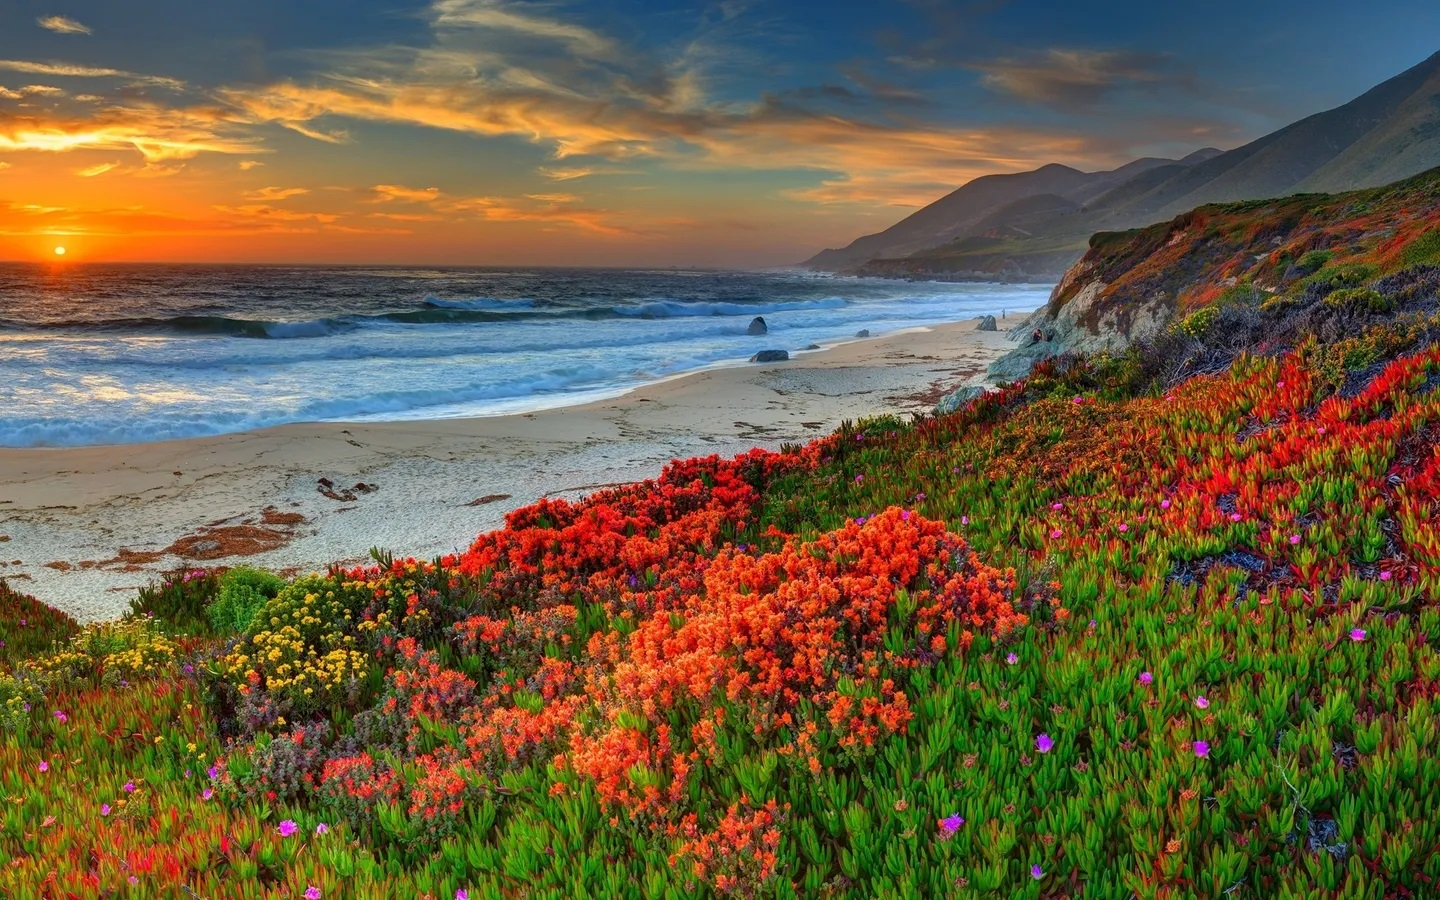
\includegraphics[width=0.9\textwidth]{figures/test.jpg}
    \bicaption{这里插入了一个普通的相片}{An ordinary photo is inserted here}
    \label{fig:my_pic1}
\end{figure}
\subsection{多图插图方法}
多图插图方法主要是用到subfloat来进行插图处理。
\begin{figure}[htbp]
    \centering
    \subfloat[泰山]{
        \begin{minipage}[t]{0.48\linewidth}
            \centering
            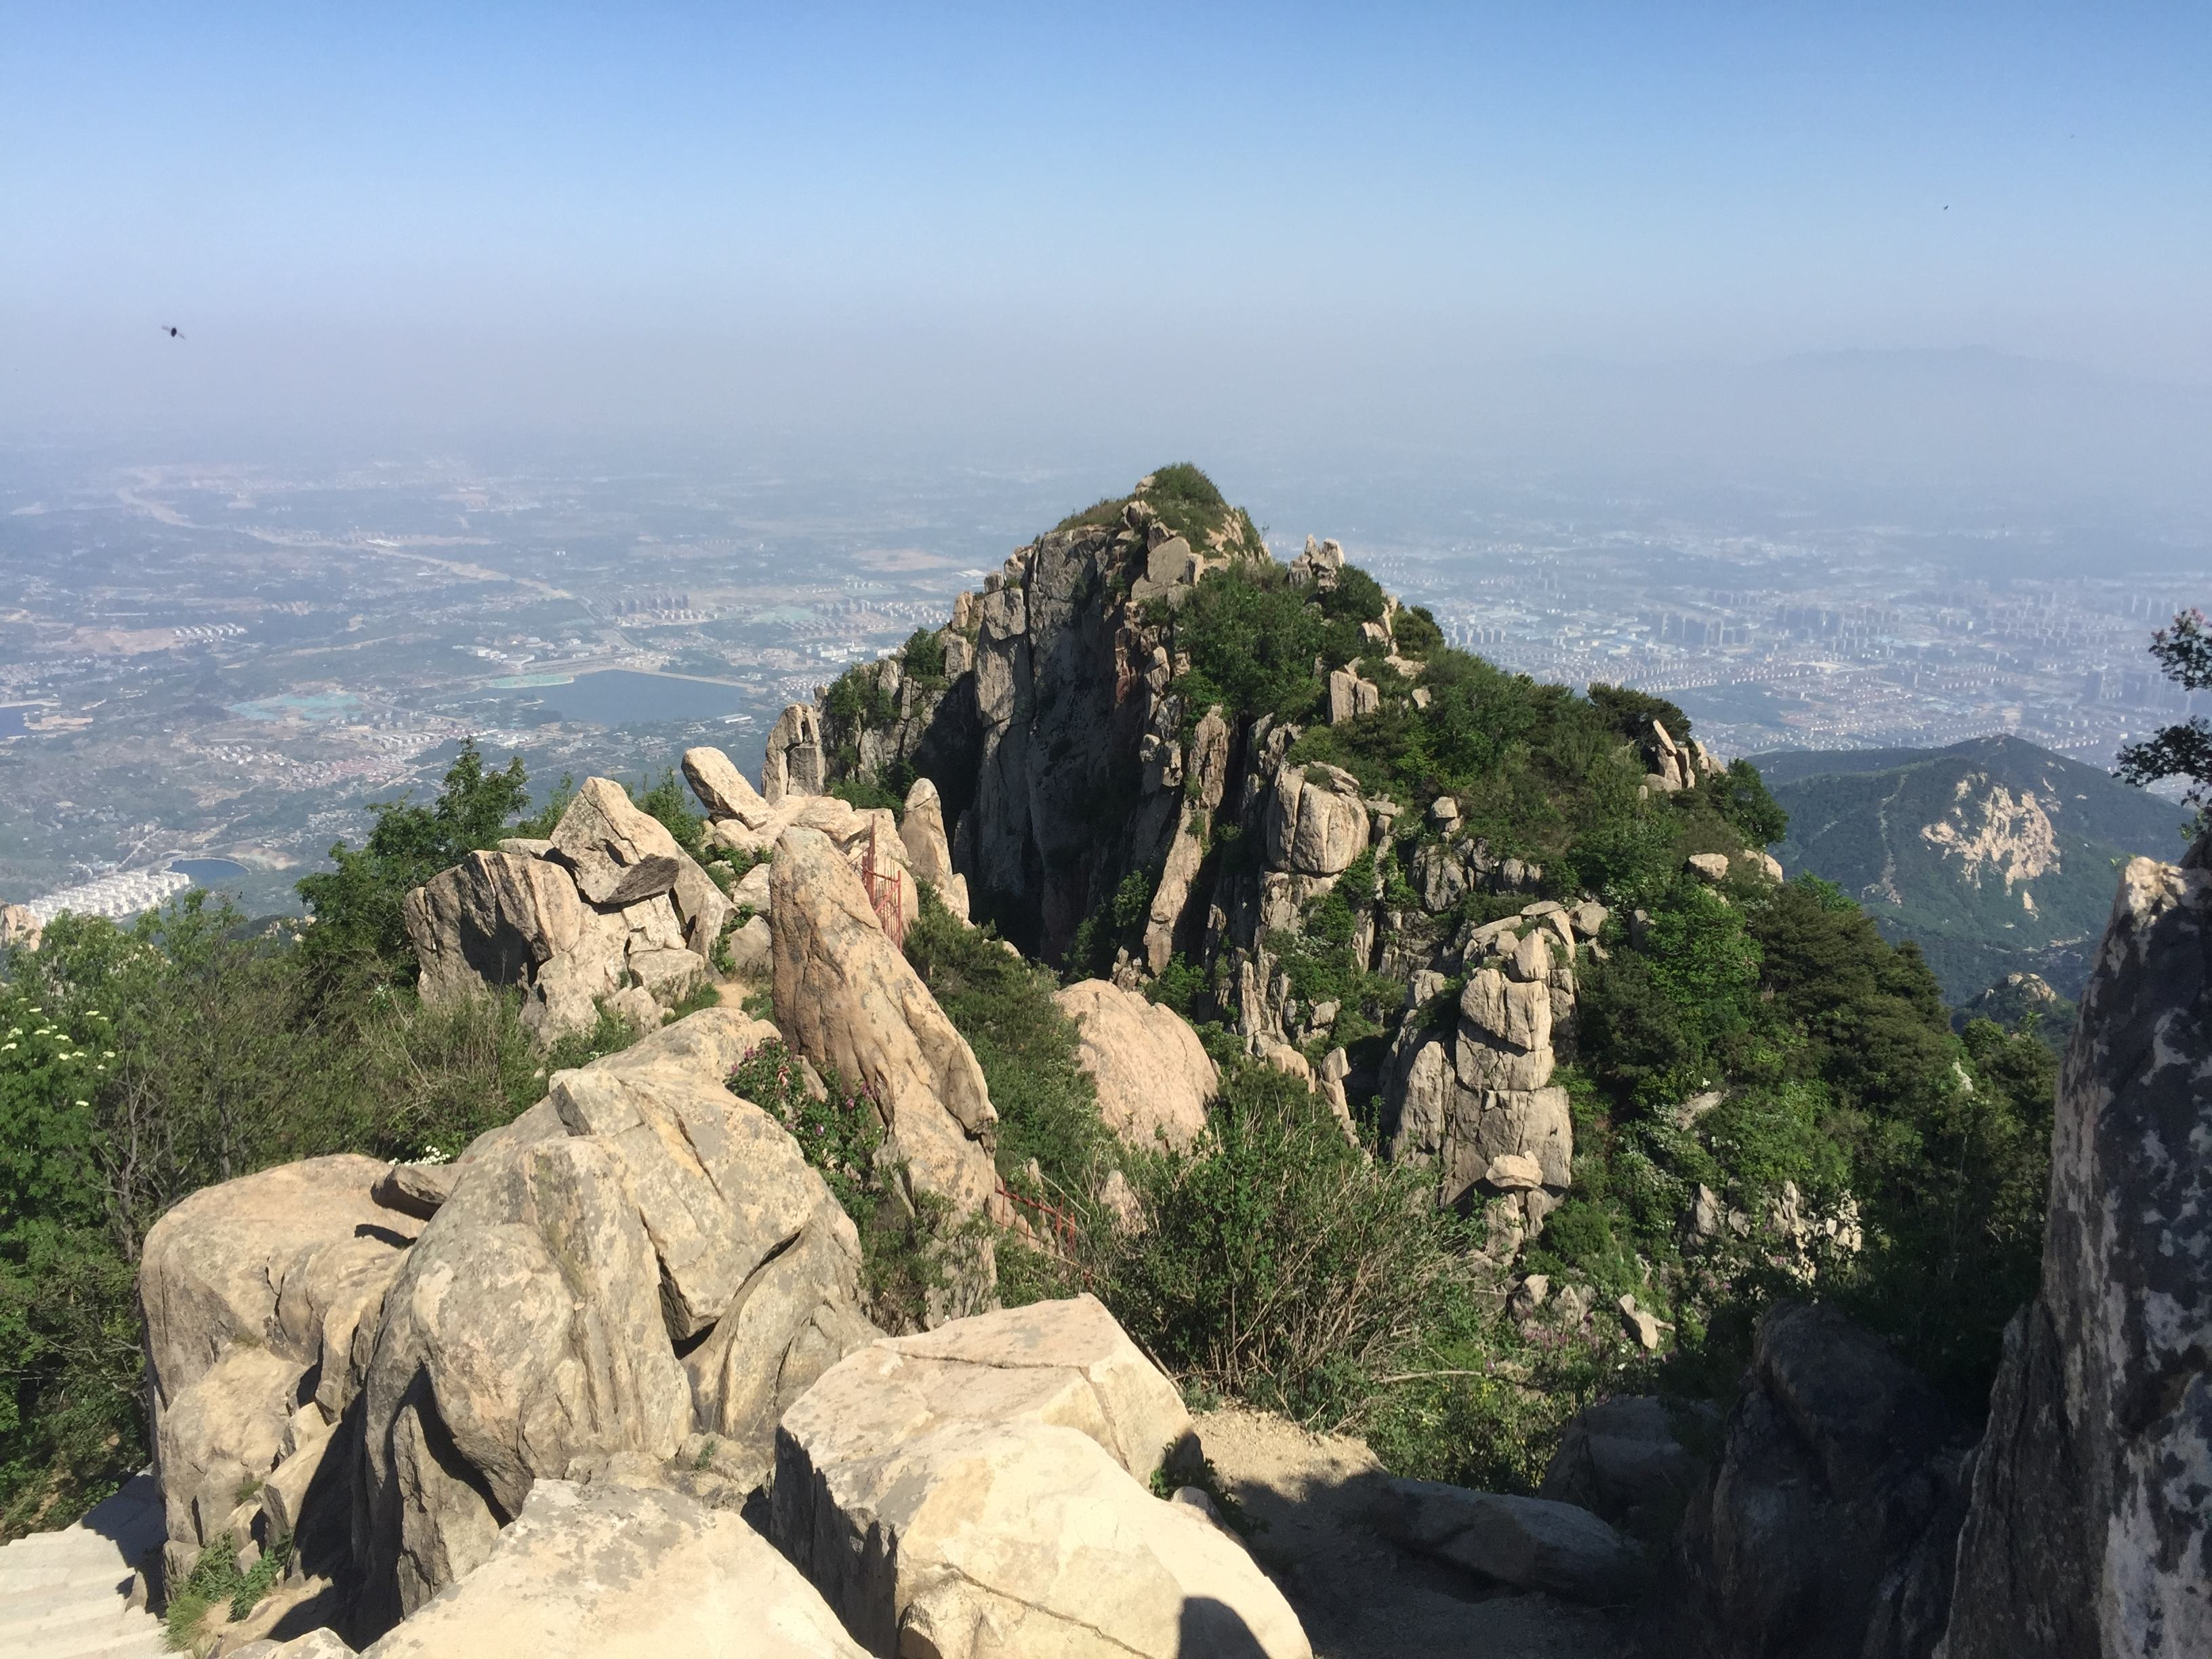
\includegraphics[width=0.9\linewidth]{figures/taishan.jpeg}
        \end{minipage}
    }\vspace{-0.1cm}
    \subfloat[桂林山水]{
        \begin{minipage}[t]{0.48\linewidth}
            \centering
            
\includegraphics[width=0.9\linewidth]{figures/guilin.jpeg}
        \end{minipage}
    }\vspace{-0.1cm}
    \subfloat[锡林郭勒盟草原]{
        \begin{minipage}[t]{0.48\linewidth}
            \centering
            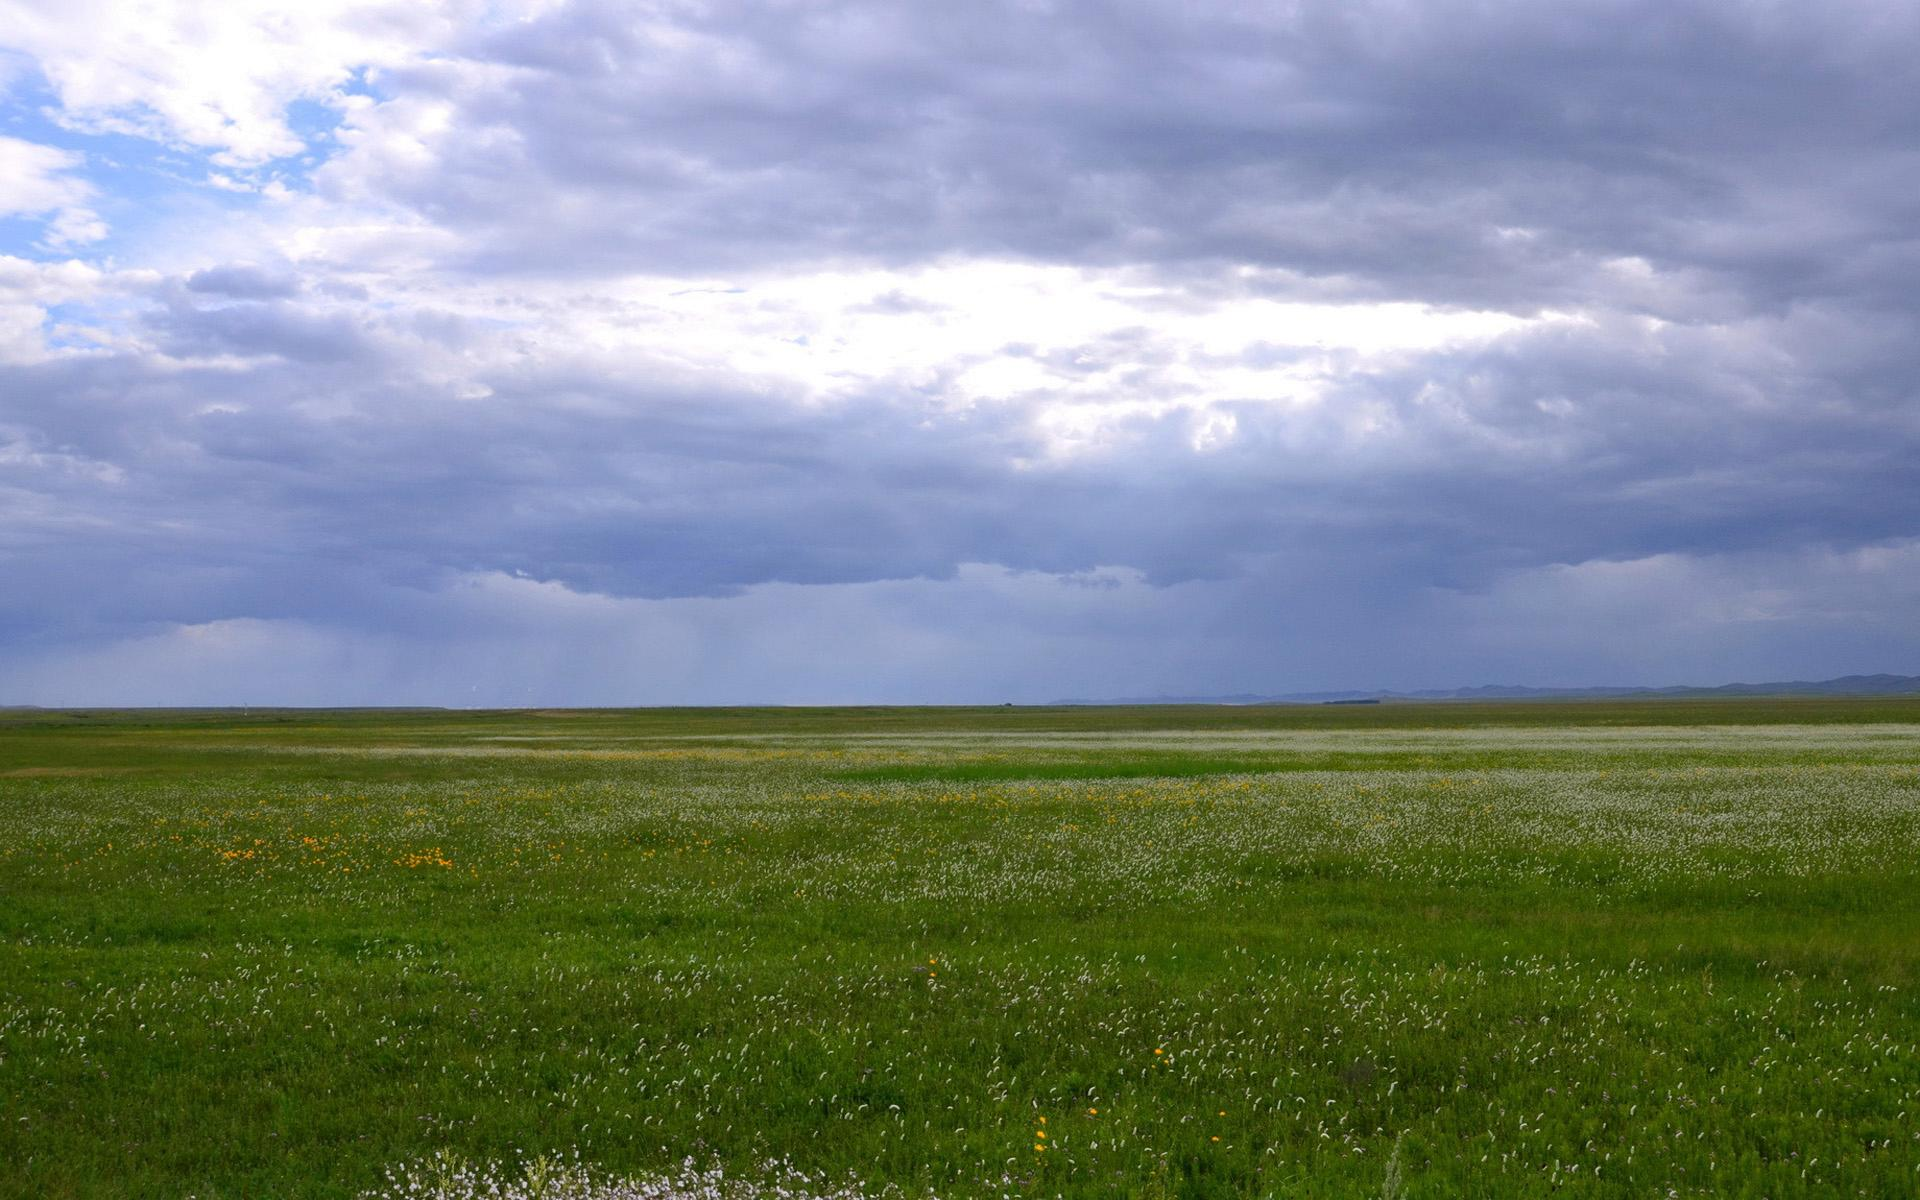
\includegraphics[width=0.9\linewidth]{figures/xilinguole.jpeg}
        \end{minipage}
    }\vspace{-0.1cm}
    \subfloat[布达拉宫]{
        \begin{minipage}[t]{0.48\linewidth}
            \centering
            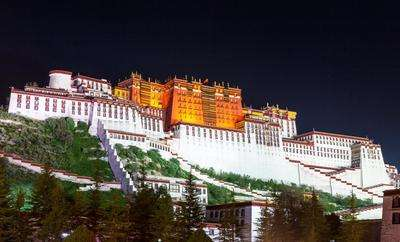
\includegraphics[width=0.9\linewidth]{figures/budalagong.jpeg}
        \end{minipage}
    }
    \centering
    \bicaption{示例的四张风景图片}{Four landscape pictures of the example}
\end{figure}

\subsection{latex自带的一些插图方法}

另外一种就是latex自带的一种画图方法,这里示例两种latex自带的画图方法。
\begin{enumerate}
    \item \textbf{复杂网络结构图}:如图\ref{fig:complex_fig}(a) 所示。
    \item \textbf{函数图像}:如图\ref{fig:complex_fig}(b),(c) 所示,详细参考\href{https://pgfplots.sourceforge.net/gallery.html},函数图像的画法使用到的是pgfplots库当中的元素画图。
\end{enumerate}

\begin{figure}
    \centering
    \subfloat[复杂网络结构图]{
        \begin{minipage}[t]{0.9\linewidth}
            \centering
            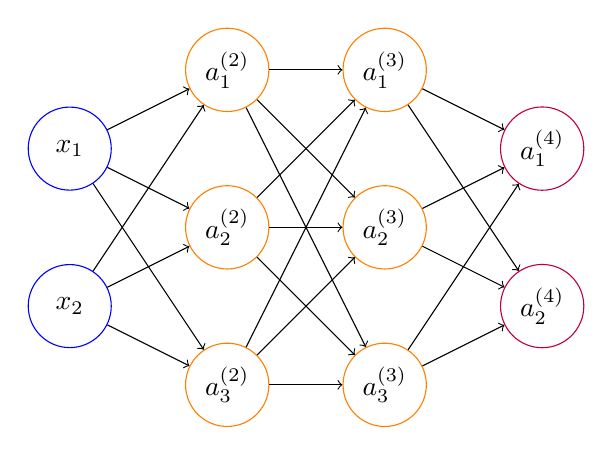
\begin{tikzpicture}
                \node[circle,
                    minimum width =30pt ,
                    minimum height =30pt ,draw=blue] (1) at(0,2){$x_1$};
                \node[circle,
                    minimum width =30pt ,
                    minimum height =30pt ,draw=blue] (2) at(0,0){$x_2$};
                \node[circle,
                    minimum width =30pt ,
                    minimum height =30pt ,draw=orange] (3) at(2,-1){$a_3^{(2)}$};
                \node[circle,
                    minimum width =30pt ,
                    minimum height =30pt ,draw=orange] (4) at(2,1){$a_2^{(2)}$};
                \node[circle,
                    minimum width =30pt ,
                    minimum height =30pt ,draw=orange] (5) at(2,3){$a_1^{(2)}$};
                \node[circle,
                    minimum width =30pt ,
                    minimum height =30pt ,draw=orange] (6) at(4,-1){$a_3^{(3)}$};
                \node[circle,
                    minimum width =30pt ,
                    minimum height =30pt ,draw=orange] (7) at(4,1){$a_2^{(3)}$};
                \node[circle,
                    minimum width =30pt ,
                    minimum height =30pt ,draw=orange] (8) at(4,3){$a_1^{(3)}$};
                \node[circle,
                    minimum width =30pt ,
                    minimum height =30pt ,draw=purple] (9) at(6,2){$a_1^{(4)}$};
                \node[circle,
                    minimum width =30pt ,
                    minimum height =30pt ,draw=purple] (10) at(6,0){$a_2^{(4)}$};
                \draw[->] (1) --(3);
                \draw[->] (1) --(4);
                \draw[->] (1) --(5);
                \draw[->] (2) --(3);
                \draw[->] (2) --(4);
                \draw[->] (2) --(5);
                \draw[->] (3) --(6);
                \draw[->] (3) --(7);
                \draw[->] (3) --(8);
                \draw[->] (4) --(6);
                \draw[->] (4) --(7);
                \draw[->] (4) --(8);
                \draw[->] (5) --(6);
                \draw[->] (5) --(7);
                \draw[->] (5) --(8);
                \draw[->] (6) --(9);
                \draw[->] (6) --(10);
                \draw[->] (7) --(9);
                \draw[->] (7) --(10);
                \draw[->] (8) --(9);
                \draw[->] (8) --(10);
            \end{tikzpicture}
        \end{minipage}
    }\vspace{-0.1cm}
    \subfloat[函数图像]{
        \begin{minipage}[t]{0.4\linewidth}
            \centering
            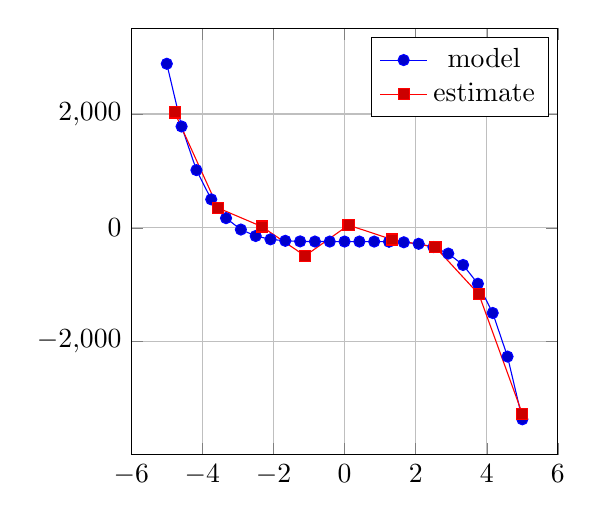
\begin{tikzpicture}
                \begin{axis}[
                    height=7cm,
                    width=7cm,
                    grid=major,
                ]
                    
                \addplot {-x^5 - 242};
                \addlegendentry{model}
            
                \addplot coordinates {
                    (-4.77778,2027.60977)
                    (-3.55556,347.84069)
                    (-2.33333,22.58953)
                    (-1.11111,-493.50066)
                    (0.11111,46.66082)
                    (1.33333,-205.56286)
                    (2.55556,-341.40638)
                    (3.77778,-1169.24780)
                    (5.00000,-3269.56775)
                };
                \addlegendentry{estimate}
                \end{axis}
            \end{tikzpicture}
        \end{minipage}
    }\vspace{-0.1cm}
    \quad
    \subfloat[统计图]{
        \begin{minipage}[t]{0.4\linewidth}
            \centering
            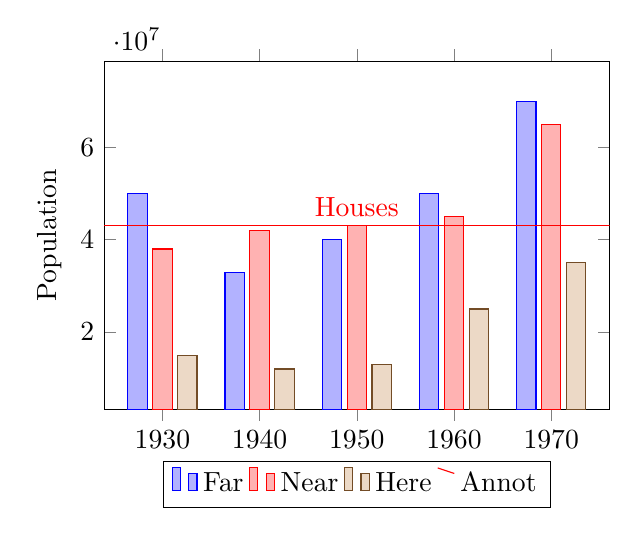
\begin{tikzpicture}
                \begin{axis}[
                    height=6cm,
                    width=8cm,
                    x tick label style={
                        /pgf/number format/1000 sep=},
                    ylabel=Population,
                    enlargelimits=0.15,
                    legend style={at={(0.5,-0.15)},
                        anchor=north,legend columns=-1},
                    ybar,
                    bar width=7pt,
                ]
                \addplot 
                    coordinates {(1930,50e6) (1940,33e6)
                         (1950,40e6) (1960,50e6) (1970,70e6)};
                
                \addplot 
                    coordinates {(1930,38e6) (1940,42e6) 
                        (1950,43e6) (1960,45e6) (1970,65e6)};
                
                \addplot 
                    coordinates {(1930,15e6) (1940,12e6) 
                        (1950,13e6) (1960,25e6) (1970,35e6)};
                
                \addplot[red,sharp plot,update limits=false] 
                    coordinates {(1910,4.3e7) (1990,4.3e7)} 
                    node[above] at (axis cs:1950,4.3e7) {Houses};
                
                \legend{Far,Near,Here,Annot}
                \end{axis}
            \end{tikzpicture}
        \end{minipage}
    }
    \bicaption{latex自带工具画图}{Drawing of latex built-in tools}
    \label{fig:complex_fig}
\end{figure}

\subsection{几个较为不错的画图例子}

使用pgfplots构建图,如\cref{fig:figure_ext1}所示。
这里给出了三个例子,分别是空间向量分布图,三维函数图像空间分布图,三角权重图。

\begin{figure}[htbp]
    \centering
    \subfloat[空间向量分布图]{
        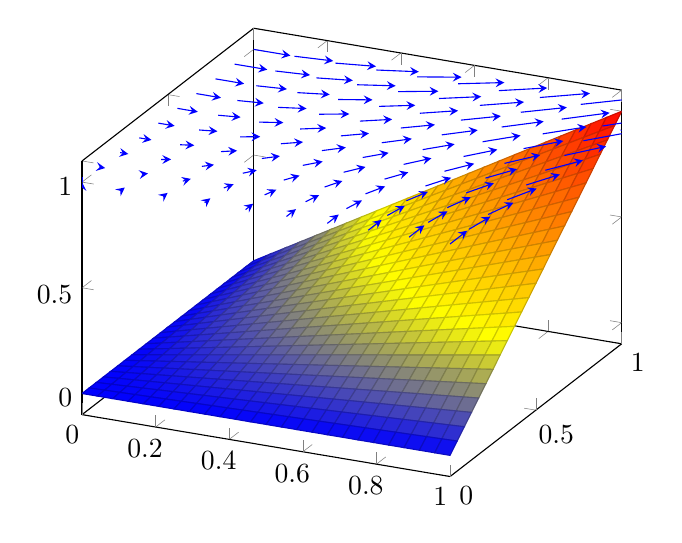
\begin{tikzpicture}
            \begin{axis}[
                domain=0:1,
                xmax=1,
                ymax=1,
            ]
            \addplot3[surf] {x*y};
            \addplot3[blue,/pgfplots/quiver,
                quiver/u=y,
                quiver/v=x,
                quiver/w=0,
                quiver/scale arrows=0.1,
                -stealth,samples=10] {1};
            \end{axis}
        \end{tikzpicture}
    }
    \subfloat[三维函数图像空间分布图]{
        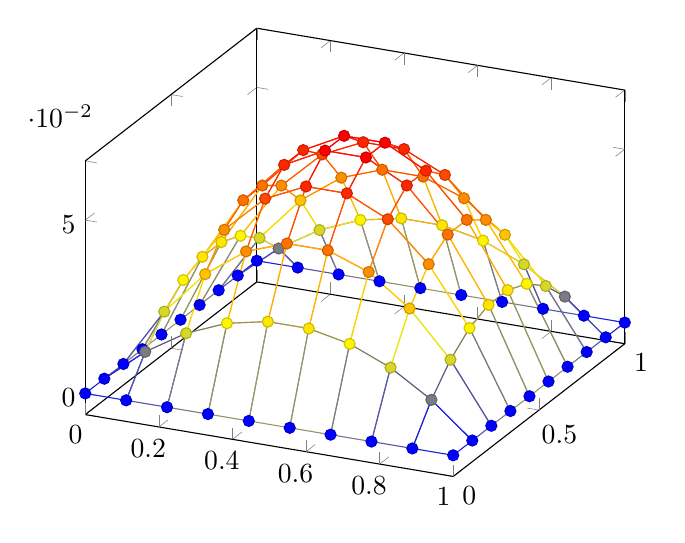
\begin{tikzpicture}
            \begin{axis}
            \addplot3+[mesh,scatter,samples=10,domain=0:1] 
                {x*(1-x)*y*(1-y)};
            \end{axis}
        \end{tikzpicture}
    }
    \quad
    \subfloat[三角权重图]{
        \begin{tikzpicture}
            \begin{ternaryaxis}[
                title=Want--be--Stainless Steel,
                xlabel=Weight Percent Chromium,
                ylabel=Weight Percent Iron,
                zlabel=Weight Percent Nickel,
                label style=sloped,
                area style,
            ]
                \addplot3 table[row sep=crcr] {
                A B C \\
                1 0 0 \\
                0.5 0.4 0.1 \\
                0.45 0.52 0.03 \\
                0.36 0.6 0.04 \\
                0.1 0.9 0 \\
                };
                \addlegendentry{Cr}
            
                \addplot3 table[row sep=crcr] {
                A B C \\
                1 0 0 \\
                0.5 0.4 0.1 \\
                0.28 0.35 0.37 \\
                0.4 0 0.6 \\
                };
                \addlegendentry{Cr+$\gamma$FeNi}
            
                \addplot3 table[row sep=crcr] {
                0.4 0 0.6 \\
                0.28 0.35 0.37 \\
                0.25 0.6 0.15 \\
                0.1 0.9 0 \\
                0 1 0 \\
                0 0 1 \\
                };
                \addlegendentry{$\gamma$FeNi}
            
                \addplot3 table[row sep=crcr] {
                0.1 0.9 0 \\
                0.36 0.6 0.04 \\
                0.25 0.6 0.15 \\
                };
                \addlegendentry{Cr+$\gamma$FeNi}
            
                \addplot3 table[row sep=crcr] {
                0.5 0.4 0.1 \\
                0.45 0.52 0.03 \\
                0.36 0.6 0.04 \\
                0.25 0.6 0.15 \\
                0.28 0.35 0.37 \\
                };
                \addlegendentry{$\sigma$+$\gamma$FeNi}
            
                \node[inner sep=0.5pt,circle,draw,fill=white,pin=-15:\footnotesize Stainless Steel] 
                  at (axis cs:0.18,0.74,0.08) {};
                
            \end{ternaryaxis}
        \end{tikzpicture}
    }
    \bicaption{几个较为不错的画图例子}{Several good examples of drawing}
    \label{fig:figure_ext1}
\end{figure}

\newpage
\subsection{神经网络图画法}
pgfplots 具有强大的功能,可以画出各种各样的图,可以画出较为不错的神经网结构图。
详细可以参考tikz网址\footnote{https://tikz.net/}以及pgfplots参考网址\footnote{https://tikz.dev/pgfplots/}\footnote{https://tikz.dev/}举个例子

\begin{figure}[hbpt]
    \centering
    % Command \empt{var1}{var2}
    \newcommand{\empt}[2]{$#1^{\langle #2 \rangle}$}
    \begin{tikzpicture}[
        % GLOBAL CFG
        font=\sf \scriptsize,
        >=LaTeX,
        % Styles
        cell/.style={% For the main box
            rectangle, 
            rounded corners=5mm, 
            draw,
            very thick,
            },
        operator/.style={%For operators like +  and  x
            circle,
            draw,
            inner sep=-0.5pt,
            minimum height =.2cm,
            },
        function/.style={%For functions
            ellipse,
            draw,
            inner sep=1pt
            },
        ct/.style={% For external inputs and outputs
            circle,
            draw,
            line width = .75pt,
            minimum width=1cm,
            inner sep=1pt,
            },
        gt/.style={% For internal inputs
            rectangle,
            draw,
            minimum width=4mm,
            minimum height=3mm,
            inner sep=1pt
            },
        mylabel/.style={% something new that I have learned
            font=\scriptsize\sffamily
            },
        ArrowC1/.style={% Arrows with rounded corners
            rounded corners=.25cm,
            thick,
            },
        ArrowC2/.style={% Arrows with big rounded corners
            rounded corners=.5cm,
            thick,
            },
        ]
    
        %Start drawing the thing...    
        % Draw the cell: 
        \node [cell, minimum height =4cm, minimum width=6cm] at (0,0){} ;
    
        % Draw inputs named ibox#
        \node [gt] (ibox1) at (-2,-0.75) {$\sigma$};
        \node [gt] (ibox2) at (-1.5,-0.75) {$\sigma$};
        \node [gt, minimum width=1cm] (ibox3) at (-0.5,-0.75) {Tanh};
        \node [gt] (ibox4) at (0.5,-0.75) {$\sigma$};
    
       % Draw opérators   named mux# , add# and func#
        \node [operator] (mux1) at (-2,1.5) {$\times$};
        \node [operator] (add1) at (-0.5,1.5) {+};
        \node [operator] (mux2) at (-0.5,0) {$\times$};
        \node [operator] (mux3) at (1.5,0) {$\times$};
        \node [function] (func1) at (1.5,0.75) {Tanh};
    
        % Draw External inputs? named as basis c,h,x
        \node[ct, label={[mylabel]Cell}] (c) at (-4,1.5) {\empt{c}{t-1}};
        \node[ct, label={[mylabel]Hidden}] (h) at (-4,-1.5) {\empt{h}{t-1}};
        \node[ct, label={[mylabel]left:Input}] (x) at (-2.5,-3) {\empt{x}{t}};
    
        % Draw External outputs? named as basis c2,h2,x2
        \node[ct, label={[mylabel]Label1}] (c2) at (4,1.5) {\empt{c}{t}};
        \node[ct, label={[mylabel]Label2}] (h2) at (4,-1.5) {\empt{h}{t}};
        \node[ct, label={[mylabel]left:Label3}] (x2) at (2.5,3) {\empt{h}{t}};
    
    % Start connecting all.
        %Intersections and displacements are used. 
        % Drawing arrows    
        \draw [ArrowC1] (c) -- (mux1) -- (add1) -- (c2);
    
        % Inputs
        \draw [ArrowC2] (h) -| (ibox4);
        \draw [ArrowC1] (h -| ibox1)++(-0.5,0) -| (ibox1); 
        \draw [ArrowC1] (h -| ibox2)++(-0.5,0) -| (ibox2);
        \draw [ArrowC1] (h -| ibox3)++(-0.5,0) -| (ibox3);
        \draw [ArrowC1] (x) -- (x |- h)-| (ibox3);
    
        % Internal
        \draw [->, ArrowC2] (ibox1) -- (mux1);
        \draw [->, ArrowC2] (ibox2) |- (mux2);
        \draw [->, ArrowC2] (ibox3) -- (mux2);
        \draw [->, ArrowC2] (ibox4) |- (mux3);
        \draw [->, ArrowC2] (mux2) -- (add1);
        \draw [->, ArrowC1] (add1 -| func1)++(-0.5,0) -| (func1);
        \draw [->, ArrowC2] (func1) -- (mux3);
    
        %Outputs
        \draw [-, ArrowC2] (mux3) |- (h2);
        \draw (c2 -| x2) ++(0,-0.1) coordinate (i1);
        \draw [-, ArrowC2] (h2 -| x2)++(-0.5,0) -| (i1);
        \draw [-, ArrowC2] (i1)++(0,0.2) -- (x2);
    
    \end{tikzpicture}
    \bicaption{LSTM 网络结构图}{LSTM network structure diagram}
\end{figure}


\begin{figure}[hbpt]
    \centering
    \definecolor{Cerulean}{RGB}{0,123,167}
    \definecolor{JungleGreen}{RGB}{0,169,154}
    \definecolor{LimeGreen}{RGB}{50, 205, 50}
    \definecolor{WildStrawberry}{RGB}{255,67,164}
    \definecolor{RedOrange}{RGB}{255, 68, 51}
    \definecolor{RubineRed}{RGB}{209, 0, 86}
    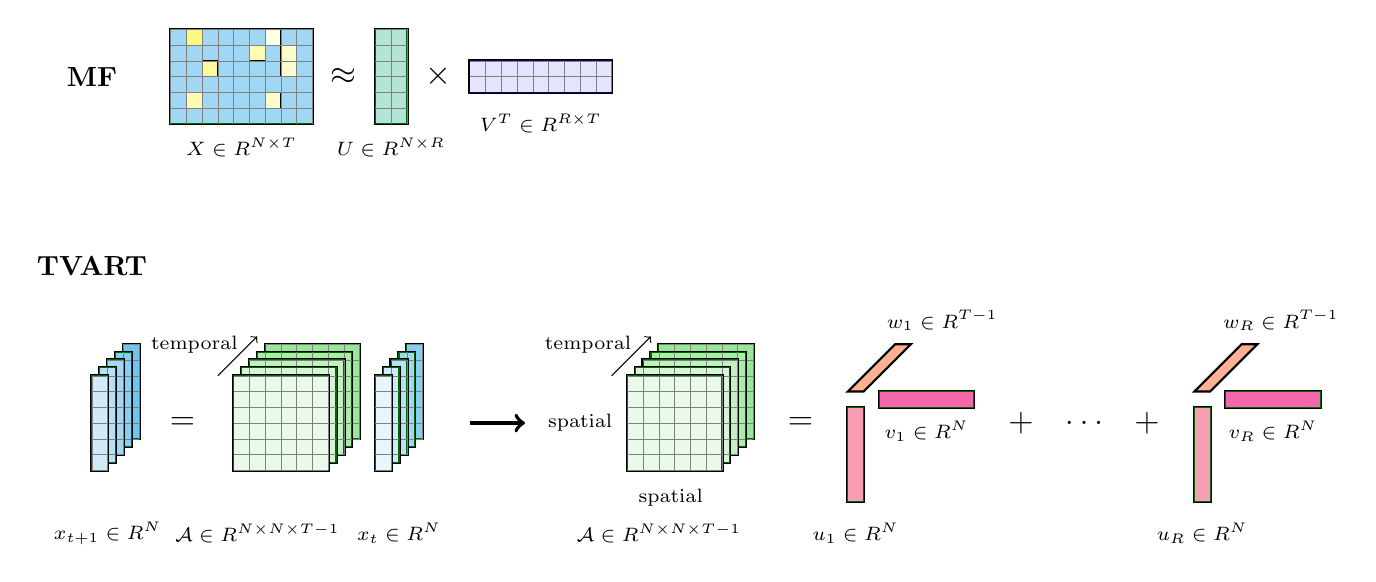
\begin{tikzpicture}
    
        % MF 
        \draw (-1,1.2) node {\textbf{MF}};
        \draw [very thick] (0,0+0.6) rectangle (3.6/2,0.6+2.4/2);
        \filldraw [fill=Cerulean!40!white,draw=green!40!black] (0,0+0.6) rectangle (3.6/2,0.6+2.4/2);
        \filldraw [fill=yellow!30] (0.4/2,0.6+0.4/2) rectangle (0.8/2,0.6+0.8/2);
        \filldraw [fill=yellow!20] (2.4/2,0.6+0.4/2) rectangle (2.8/2,0.6+0.8/2);
        \filldraw [fill=yellow!40] (0.8/2,0.6+1.2/2) rectangle (1.2/2,0.6+1.6/2);
        \filldraw [fill=yellow!30] (2.0/2,0.6+1.6/2) rectangle (2.4/2,0.6+2.0/2);
        \filldraw [fill=yellow!50] (0.4/2,0.6+2.0/2) rectangle (0.8/2,0.6+2.4/2);
        \filldraw [fill=yellow!10] (2.4/2,0.6+2.0/2) rectangle (2.8/2,0.6+2.4/2);
        \filldraw [fill=yellow!20] (2.8/2,0.6+1.2/2) rectangle (3.2/2,0.6+2.0/2);
        \draw [step=0.4/2, very thin, color=gray] (0,0.6) grid (3.6/2,0.6+2.4/2);
        \draw (1.8/2,-0.3+0.6) node {{\color{black}\scriptsize{$X\in\mathbb{R}^{N\times T}$}}};
        
        % U
        \draw (4.4/2,1.2/2+0.6) node {{\color{black}\large{$\approx$}}};
        \draw [very thick] (5.2/2,0+0.6) rectangle (6.0/2,2.4/2+0.6);
        \filldraw [fill=JungleGreen!30!white,draw=green!40!black] (5.2/2,0+0.6) rectangle (6.0/2,2.4/2+0.6);
        \draw [step=0.4/2, very thin, color=gray] (5.2/2,0+0.6) grid (6.0/2,2.4/2+0.6);
        \draw (5.6/2,-0.3+0.6) node {{\color{black}\scriptsize{$U\in\mathbb{R}^{N\times R}$}}};
        
        % V
        \draw (6.8/2,1.2/2+0.6) node {{\color{black}\large{$\times$}}};
        \draw [very thick] (7.6/2,0.8/2+0.6) rectangle (11.2/2,1.6/2+0.6);
        \filldraw [fill=blue!10!white,draw=blue!40!black] (7.6/2,0.8/2+0.6) rectangle (11.2/2,1.6/2+0.6);
        \draw [step=0.4/2, very thin, color=gray] (7.6/2,0.8/2+0.6) grid (11.2/2,1.6/2+0.6);
        \draw (9.4/2,0+0.6) node {{\color{black}\scriptsize{$V^{T}\in\mathbb{R}^{R\times T}$}}};
        
        % TVART MODEL
        \draw (-1,-1.2) node {\textbf{TVART}};
        
        
        % AR MODEL
        \draw [very thick] (.8+0.4,-3.8+0.4) rectangle (2+0.4,-2.6+0.4);
        \filldraw [fill=LimeGreen!50!white,draw=green!40!black] (.8+0.4,-3.8+0.4) rectangle (2+0.4,-2.6+0.4);
        \draw [step=0.4/2, very thin, color=gray] (.8+0.4,-3.8+0.4) grid (2+0.4,-2.6+0.4);
        
        \draw [very thick] (.8+0.3,-3.8+0.3) rectangle (2+0.3,-2.6+0.3);
        \filldraw [fill=LimeGreen!40!white,draw=green!40!black] (.8+0.3,-3.8+0.3) rectangle (2+0.3,-2.6+0.3);
        \draw [step=0.4/2, very thin, color=gray] (.8+0.3,-3.8+0.3) grid (2+0.3,-2.6+0.3);
        
        \draw [very thick] (.8+0.2,-3.8+0.2) rectangle (2+0.2,-2.6+0.2);
        \filldraw [fill=LimeGreen!30!white,draw=green!40!black] (.8+0.2,-3.8+0.2) rectangle (2+0.2,-2.6+0.2);
        \draw [step=0.4/2, very thin, color=gray] (.8+0.2,-3.8+0.2) grid (2+0.2,-2.6+0.2);
        
        \draw [very thick] (.8+0.1,-3.8+0.1) rectangle (2+0.1,-2.6+0.1);
        \filldraw [fill=LimeGreen!20!white,draw=green!40!black] (.8+0.1,-3.8+0.1) rectangle (2+0.1,-2.6+0.1);
        \draw [step=0.4/2, very thin, color=gray] (.8+0.1,-3.8+0.1) grid (2+0.1,-2.6+0.1);
        
        \draw [very thick] (.8,-3.8) rectangle (2,-2.6);
        \filldraw [fill=LimeGreen!10!white,draw=green!40!black] (.8,-3.8) rectangle (2,-2.6);
        \draw [step=0.4/2, very thin, color=gray] (.8,-3.8) grid (2,-2.6);
        
          \draw (1.1,-4.6) node
        {{\color{black}\scriptsize{$\mathcal{A}\in\mathbb{R}^{N \times N \times T-1}$}}};
        % y vector
    
        \draw [very thick] (0+0.4-0.8-0.2,-3.8+0.4) rectangle (0.2+0.4-0.8-0.2,-2.6+0.4);
        \filldraw [fill=Cerulean!60!white,draw=green!40!black] (0+0.4-0.8-0.2,-3.8+0.4) rectangle (0.2+0.4-0.8-0.2,-2.6+0.4);
        \draw [step=0.4/2, very thin, color=gray] (0+0.4-0.8-0.2,-3.8+0.4) grid (0.2+0.4-0.8-0.2,-2.6+0.4);
        
        \draw [very thick] (0+0.3-0.8-0.2,-3.8+0.3) rectangle (0.2+0.3-0.8-0.2,-2.6+0.3);
        \filldraw [fill=Cerulean!50!white,draw=green!40!black] (0+0.3-0.8-0.2,-3.8+0.3) rectangle (0.2+0.3-0.8-0.2,-2.6+0.3);
        \draw [step=0.4/2, very thin, color=gray] (0+0.3-0.8-0.2,-3.8+0.3) grid (0.2+0.3-0.8-0.2,-2.6+0.3);
    
        \draw [very thick] (0+0.2-0.8-0.2,-3.8+0.2) rectangle (0.2+0.2-0.8-0.2,-2.6+0.2);
        \filldraw [fill=Cerulean!40!white,draw=green!40!black] (0+0.2-0.8-0.2,-3.8+0.2) rectangle (0.2+0.2-0.8-0.2,-2.6+0.2);
        \draw [step=0.4/2, very thin, color=gray] (0+0.2-0.8-0.2,-3.8+0.2) grid (0.2+0.2-0.8-0.2,-2.6+0.2);
        
        \draw [very thick] (0.1-0.8-0.2,-3.8+0.1) rectangle (0.2+0.1-0.8-0.2,-2.6+0.1);
        \filldraw [fill=Cerulean!30!white,draw=green!40!black] (0+0.1-0.8-0.2,-3.8+0.1) rectangle (0.2+0.1-0.8-0.2,-2.6+0.1);
        \draw [step=0.4/2, very thin, color=gray] (0+0.1-0.8-0.2,-3.8+0.1) grid (0.2+0.1-0.8-0.2,-2.6+0.1);
        
        \draw [very thick] (0-0.8-0.2,-3.8) rectangle (0.2-0.8-0.2,-2.6);
        \filldraw [fill=Cerulean!20!white,draw=green!40!black] (0-0.8-0.2,-3.8) rectangle (0.2-0.8-0.2,-2.6);
        \draw [step=0.4/2, very thin, color=gray] (0-0.8-0.2,-3.8) grid (0.2-0.8-0.2,-2.6);
        \draw (0-0.8,-4.6) node {{\color{black}\scriptsize{$\boldsymbol{x}_{t+1}\in\mathbb{R}^{N}$}}};
        
        \draw (0.15,-3.2) node {{\color{black}\large{$=$}}};
        % x vector
        \draw [very thick] (0+0.4+2.6,-3.8+0.4) rectangle (0.2+0.4+2.6,-2.6+0.4);
        \filldraw [fill=Cerulean!50!white,draw=green!40!black] (0+0.4+2.6,-3.8+0.4) rectangle (0.2+0.4+2.6,-2.6+0.4);
        \draw [step=0.4/2, very thin, color=gray] (0+0.4+2.6,-3.8+0.4) grid (0.2+0.4+2.6,-2.6+0.4);
        
        \draw [very thick] (0+0.3+2.6,-3.8+0.3) rectangle (0.2+0.3+2.6,-2.6+0.3);
        \filldraw [fill=Cerulean!40!white,draw=green!40!black] (0+0.3+2.6,-3.8+0.3) rectangle (0.2+0.3+2.6,-2.6+0.3);
        \draw [step=0.4/2, very thin, color=gray] (0+0.3+2.6,-3.8+0.3) grid (0.2+0.3+2.6,-2.6+0.3);
    
        \draw [very thick] (0+0.2+2.6,-3.8+0.2) rectangle (0.2+0.2+2.6,-2.6+0.2);
        \filldraw [fill=Cerulean!30!white,draw=green!40!black] (0+0.2+2.6,-3.8+0.2) rectangle (0.2+0.2+2.6,-2.6+0.2);
        \draw [step=0.4/2, very thin, color=gray] (0+0.2+2.6,-3.8+0.2) grid (0.2+0.2+2.6,-2.6+0.2);
        
        \draw [very thick] (0.1+2.6,-3.8+0.1) rectangle (0.2+0.1+2.6,-2.6+0.1);
        \filldraw [fill=Cerulean!20!white,draw=green!40!black] (0+0.1+2.6,-3.8+0.1) rectangle (0.2+0.1+2.6,-2.6+0.1);
        \draw [step=0.4/2, very thin, color=gray] (0+0.1+2.6,-3.8+0.1) grid (0.2+0.1+2.6,-2.6+0.1);
        
        \draw [very thick] (0+2.6,-3.8) rectangle (0.2+2.6,-2.6);
        \filldraw [fill=Cerulean!10!white,draw=green!40!black] (0+2.6,-3.8) rectangle (0.2+2.6,-2.6);
        \draw [step=0.4/2, very thin, color=gray] (0+2.6,-3.8) grid (0.2+2.6,-2.6);
        
        \draw (2.9 ,-4.6) node {{\color{black}\scriptsize{$\boldsymbol{x}_{t}\in\mathbb{R}^{N}$}}};
    
        \draw[->] (0.6,-2.6) -- (1.1,-2.1);
        \draw (0.3,-2.2) node {{\color{black}\scriptsize{temporal}}};
    
        \draw[->, line width=0.5mm] (3.8,-3.2) -- (4.5,-3.2);
        
        % tensor A
        \draw [very thick] (5.8+0.4,-3.8+0.4) rectangle (7+0.4,-2.6+0.4);
        \filldraw [fill=LimeGreen!50!white,draw=green!40!black] (5.8+0.4,-3.8+0.4) rectangle (7+0.4,-2.6+0.4);
        \draw [step=0.4/2, very thin, color=gray] (5.8+0.4,-3.8+0.4) grid (7+0.4,-2.6+0.4);
        
        \draw [very thick] (5.8+0.3,-3.8+0.3) rectangle (7+0.3,-2.6+0.3);
        \filldraw [fill=LimeGreen!40!white,draw=green!40!black] (5.8+0.3,-3.8+0.3) rectangle (7+0.3,-2.6+0.3);
        \draw [step=0.4/2, very thin, color=gray] (5.8+0.3,-3.8+0.3) grid (7+0.3,-2.6+0.3);
        
        \draw [very thick] (5.8+0.2,-3.8+0.2) rectangle (7+0.2,-2.6+0.2);
        \filldraw [fill=LimeGreen!30!white,draw=green!40!black] (5.8+0.2,-3.8+0.2) rectangle (7+0.2,-2.6+0.2);
        \draw [step=0.4/2, very thin, color=gray] (5.8+0.2,-3.8+0.2) grid (7+0.2,-2.6+0.2);
        
        \draw [very thick] (5.8+0.1,-3.8+0.1) rectangle (7+0.1,-2.6+0.1);
        \filldraw [fill=LimeGreen!20!white,draw=green!40!black] (5.8+0.1,-3.8+0.1) rectangle (7+0.1,-2.6+0.1);
        \draw [step=0.4/2, very thin, color=gray] (5.8+0.1,-3.8+0.1) grid (7+0.1,-2.6+0.1);
        
        \draw [very thick] (5.8,-3.8) rectangle (7,-2.6);
        \filldraw [fill=LimeGreen!10!white,draw=green!40!black] (5.8,-3.8) rectangle (7,-2.6);
        \draw [step=0.4/2, very thin, color=gray] (5.8,-3.8) grid (7,-2.6);
        \draw[->] (5.6,-2.6) -- (6.1,-2.1);
        
        \draw (6.35,-4.15) node {{\color{black}\scriptsize{spatial}}};
        \draw (5.2,-3.2) node {{\color{black}\scriptsize{spatial}}};
        \draw (5.3,-2.2) node {{\color{black}\scriptsize{temporal}}};
        
        \draw (6.2,-4.6) node {{\color{black}\scriptsize{$\mathcal{A}\in\mathbb{R}^{N \times N \times T-1}$}}};
      
        \draw (8,-3.2) node {{\color{black}\large{$=$}}};
    
        % CP 
        \draw [very thick] (8.6,-4.4+0.2) rectangle (8.8,-3.2+0.2);
        \filldraw [fill=WildStrawberry!40!white,draw=green!40!black] (8.6,-4.4+0.2) rectangle (8.8,-3.2+0.2);
        \draw (8.7,-4.8+0.2) node {{\color{black}\scriptsize{$\boldsymbol{u}_1 \in \mathbb{R}^N$}}};
        
        \draw [very thick] (9,-3-0.2+0.2) rectangle (10.2,-2.8-0.2+0.2);
        \filldraw [fill=RubineRed!60!white,draw=green!40!black] (9,-3-0.2+0.2) rectangle (10.2,-2.8-0.2+0.2);
        \draw (9.6,-3.3-0.2+0.2) node {{\color{black}\scriptsize{$\boldsymbol{v}_1 \in \mathbb{R}^N$}}};
        
    
        \draw[fill=RedOrange!40!white, line width=0.8pt] (9.2,-2.4+0.2) -- (9.4,-2.4+0.2) -- (8.8,-3+0.2) -- (8.6,-3+0.2) -- cycle;
        \draw (10-0.2,-1.9) node {{\color{black}\scriptsize{$\boldsymbol{w}_1 \in \mathbb{R}^{T-1}$}}};
    
        \draw (10.8,-3.2) node {{\color{black}\large{$+$}}};
        \draw (11.6,-3.2) node {{\color{black}\large{$\dots$}}};
        \draw (12.4,-3.2) node {{\color{black}\large{$+$}}};
        
        \draw [very thick] (8.6+4.4,-4.4+0.2) rectangle (8.8+4.4,-3.2+0.2);
        \filldraw [fill=WildStrawberry!40!white,draw=green!40!black] (8.6+4.4,-4.4+0.2) rectangle (8.8+4.4,-3.2+0.2);
        \draw (8.7+4.4,-4.8+0.2) node {{\color{black}\scriptsize{$\boldsymbol{u}_R \in \mathbb{R}^N $}}};
        
        \draw [very thick] (9+4.4,-3-0.2+0.2) rectangle (10.2+4.4,-2.8-0.2+0.2);
        \filldraw [fill=RubineRed!60!white,draw=green!40!black] (9+4.4,-3-0.2+0.2) rectangle (10.2+4.4,-2.8-0.2+0.2);
        \draw (9.6+4.4,-3.3-0.2+0.2) node {{\color{black}\scriptsize{$\boldsymbol{v}_R\in \mathbb{R}^N$}}};
        
        \draw[fill=RedOrange!40!white, line width=0.8pt] (9.2+4.4,-2.4+0.2) -- (9.4+4.4,-2.4+0.2) -- (8.8+4.4,-3+0.2) -- (8.6+4.4,-3+0.2) -- cycle;
        \draw (10.1+4,-1.9) node {{\color{black}\scriptsize{$\boldsymbol{w}_R\in \mathbb{R}^{T-1}$}}};
        
    \end{tikzpicture}
    \bicaption{张量分解模型}{Tensor decomposition model}
    \label{fig:tensor}
\end{figure}


\begin{figure}[t!]
	\centering
	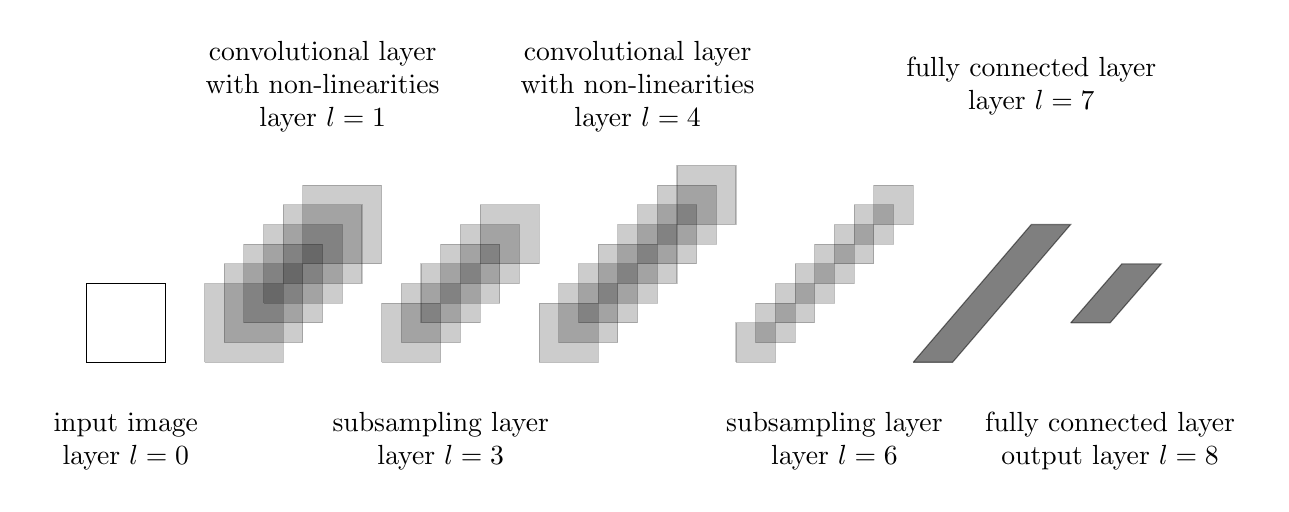
\begin{tikzpicture}
		\node at (0.5,-1){\begin{tabular}{c}input image\\layer $l = 0$\end{tabular}};
		
		\draw (0,0) -- (1,0) -- (1,1) -- (0,1) -- (0,0);
		
		\node at (3,3.5){\begin{tabular}{c}convolutional layer\\with non-linearities\\layer $l = 1$\end{tabular}};
		
		\draw[fill=black,opacity=0.2,draw=black] (2.75,1.25) -- (3.75,1.25) -- (3.75,2.25) -- (2.75,2.25) -- (2.75,1.25);
		\draw[fill=black,opacity=0.2,draw=black] (2.5,1) -- (3.5,1) -- (3.5,2) -- (2.5,2) -- (2.5,1);
		\draw[fill=black,opacity=0.2,draw=black] (2.25,0.75) -- (3.25,0.75) -- (3.25,1.75) -- (2.25,1.75) -- (2.25,0.75);
		\draw[fill=black,opacity=0.2,draw=black] (2,0.5) -- (3,0.5) -- (3,1.5) -- (2,1.5) -- (2,0.5);
		\draw[fill=black,opacity=0.2,draw=black] (1.75,0.25) -- (2.75,0.25) -- (2.75,1.25) -- (1.75,1.25) -- (1.75,0.25);
		\draw[fill=black,opacity=0.2,draw=black] (1.5,0) -- (2.5,0) -- (2.5,1) -- (1.5,1) -- (1.5,0);
		
		\node at (4.5,-1){\begin{tabular}{c}subsampling layer\\layer $l = 3$\end{tabular}};
		
		\draw[fill=black,opacity=0.2,draw=black] (5,1.25) -- (5.75,1.25) -- (5.75,2) -- (5,2) -- (5,1.25);
		\draw[fill=black,opacity=0.2,draw=black] (4.75,1) -- (5.5,1) -- (5.5,1.75) -- (4.75,1.75) -- (4.75,1);
		\draw[fill=black,opacity=0.2,draw=black] (4.5,0.75) -- (5.25,0.75) -- (5.25,1.5) -- (4.5,1.5) -- (4.5,0.75);
		\draw[fill=black,opacity=0.2,draw=black] (4.25,0.5) -- (5,0.5) -- (5,1.25) -- (4.25,1.25) -- (4.25,0.5);
		\draw[fill=black,opacity=0.2,draw=black] (4,0.25) -- (4.75,0.25) -- (4.75,1) -- (4,1) -- (4,0.25);
		\draw[fill=black,opacity=0.2,draw=black] (3.75,0) -- (4.5,0) -- (4.5,0.75) -- (3.75,0.75) -- (3.75,0);
		
		\node at (7,3.5){\begin{tabular}{c}convolutional layer\\with non-linearities\\layer $l = 4$\end{tabular}};
		
		\draw[fill=black,opacity=0.2,draw=black] (7.5,1.75) -- (8.25,1.75) -- (8.25,2.5) -- (7.5,2.5) -- (7.5,1.75);
		\draw[fill=black,opacity=0.2,draw=black] (7.25,1.5) -- (8,1.5) -- (8,2.25) -- (7.25,2.25) -- (7.25,1.5);
		\draw[fill=black,opacity=0.2,draw=black] (7,1.25) -- (7.75,1.25) -- (7.75,2) -- (7,2) -- (7,1.25);
		\draw[fill=black,opacity=0.2,draw=black] (6.75,1) -- (7.5,1) -- (7.5,1.75) -- (6.75,1.75) -- (6.75,1);
		\draw[fill=black,opacity=0.2,draw=black] (6.5,0.75) -- (7.25,0.75) -- (7.25,1.5) -- (6.5,1.5) -- (6.5,0.75);
		\draw[fill=black,opacity=0.2,draw=black] (6.25,0.5) -- (7,0.5) -- (7,1.25) -- (6.25,1.25) -- (6.25,0.5);
		\draw[fill=black,opacity=0.2,draw=black] (6,0.25) -- (6.75,0.25) -- (6.75,1) -- (6,1) -- (6,0.25);
		\draw[fill=black,opacity=0.2,draw=black] (5.75,0) -- (6.5,0) -- (6.5,0.75) -- (5.75,0.75) -- (5.75,0);
		
		\node at (9.5,-1){\begin{tabular}{c}subsampling layer\\layer $l = 6$\end{tabular}};
		
		\draw[fill=black,opacity=0.2,draw=black] (10,1.75) -- (10.5,1.75) -- (10.5,2.25) -- (10,2.25) -- (10,1.75);
		\draw[fill=black,opacity=0.2,draw=black] (9.75,1.5) -- (10.25,1.5) -- (10.25,2) -- (9.75,2) -- (9.75,1.5);
		\draw[fill=black,opacity=0.2,draw=black] (9.5,1.25) -- (10,1.25) -- (10,1.75) -- (9.5,1.75) -- (9.5,1.25);
		\draw[fill=black,opacity=0.2,draw=black] (9.25,1) -- (9.75,1) -- (9.75,1.5) -- (9.25,1.5) -- (9.25,1);
		\draw[fill=black,opacity=0.2,draw=black] (9,0.75) -- (9.5,0.75) -- (9.5,1.25) -- (9,1.25) -- (9,0.75);
		\draw[fill=black,opacity=0.2,draw=black] (8.75,0.5) -- (9.25,0.5) -- (9.25,1) -- (8.75,1) -- (8.75,0.5);
		\draw[fill=black,opacity=0.2,draw=black] (8.5,0.25) -- (9,0.25) -- (9,0.75) -- (8.5,0.75) -- (8.5,0.25);
		\draw[fill=black,opacity=0.2,draw=black] (8.25,0) -- (8.75,0) -- (8.75,0.5) -- (8.25,0.5) -- (8.25,0);
		
		\node at (12,3.5){\begin{tabular}{c}fully connected layer\\layer $l = 7$\end{tabular}};
		
		\draw[fill=black,draw=black,opacity=0.5] (10.5,0) -- (11,0) -- (12.5,1.75) -- (12,1.75) -- (10.5,0);
		
		\node at (13,-1){\begin{tabular}{c}fully connected layer\\output layer $l = 8$\end{tabular}};
		
		\draw[fill=black,draw=black,opacity=0.5] (12.5,0.5) -- (13,0.5) -- (13.65,1.25) -- (13.15,1.25) -- (12.5,0.5);
	\end{tikzpicture}
	\bicaption{传统LeNet-5卷积神经网络结构图}{Traditional LeNet-5 convolutional neural network structure diagram}
	\label{fig:traditional-convolutional-network}
\end{figure}


\begin{figure}[hbpt]
    \centering
    \begin{tikzpicture}[
        ->, thick,
        node/.style={circle, fill=teal!60},
        label/.style={below, font=\footnotesize},
      ]
    
      \node[node] (zin) {$\vec z_\text{in}$};
      \node[node, right=5em of zin] (fake) {$\vec x_\text{fake}$};
      \draw (zin) -- node[above] {$G(\vec x)$} node[label] {generator} (fake);
    
      \draw[<-] (zin) -- node[above] {$p_\theta(\vec z)$} node[label] {latent noise} ++(-3,0);
      \node[node, above=of fake] (real) {$\vec x_\text{real}$};
      \draw[<-] (real) -- node[above] {$p_\text{data}(\vec x)$} ++(-3,0);
      \node[node, right=6em of fake] (D) at ($(fake)!0.5!(real)$) {$\vec x$};
      \node[right=7em of D] (out) {real?};
      \draw (D) -- node[above] {$D(\vec x)$} node[label] {discriminator} (out);
    
      \coordinate[right=2.5em of fake, circle, fill, inner sep=0.15em] (pt1);
      \coordinate[right=2.5em of real, circle, fill, inner sep=0.15em] (pt2);
    
      \draw[-, dashed] (pt1) edge[bend left] coordinate[circle, fill=orange, inner sep=1mm, pos=0.7] (pt3) (pt2);
      \draw (fake) -- (pt1) (real) -- (pt2) (pt3) -- (D);
    
    \end{tikzpicture}
    \bicaption{GAN的示意图}{Illustration of GAN}
    \label{fig:gan_network}
\end{figure}

\begin{figure}
    \begin{tikzpicture}[scale=.9,every node/.style={minimum size=1cm},on grid]
        %slanting: production of a set of n 'laminae' to be piled up. N=number of grids.
        \begin{scope}[
                yshift=-83,every node/.append style={
                yslant=0.5,xslant=-1},yslant=0.5,xslant=-1
                ]
            % opacity to prevent graphical interference
            \fill[white,fill opacity=0.9] (0,0) rectangle (5,5);
            \draw[step=4mm, black] (0,0) grid (5,5); %defining grids
            \draw[step=1mm, red!50,thin] (3,1) grid (4,2);  %Nested Grid
            \draw[black,very thick] (0,0) rectangle (5,5);%marking borders
            \fill[red] (0.05,0.05) rectangle (0.35,0.35);
            %Idem as above, for the n-th grid:
        \end{scope}
            
        \begin{scope}[
            yshift=0,every node/.append style={
                yslant=0.5,xslant=-1},yslant=0.5,xslant=-1
                         ]
            \fill[white,fill opacity=.9] (0,0) rectangle (5,5);
            \draw[black,very thick] (0,0) rectangle (5,5);
            \draw[step=5mm, black] (0,0) grid (5,5);
        \end{scope}
            
        \begin{scope}[
            yshift=90,every node/.append style={
            yslant=0.5,xslant=-1},yslant=0.5,xslant=-1
                         ]
            \fill[white,fill opacity=.9] (0,0) rectangle (5,5);
            \draw[step=10mm, black] (1,1) grid (4,4);
            \draw[black,very thick] (1,1) rectangle (4,4);
            \draw[black,dashed] (0,0) rectangle (5,5);
        \end{scope}
            
        \begin{scope}[
            yshift=170,every node/.append style={
                yslant=0.5,xslant=-1},yslant=0.5,xslant=-1
              ]
            \fill[white,fill opacity=0.6] (0,0) rectangle (5,5);
            \draw[step=10mm, black] (2,2) grid (5,5);
            \draw[step=2mm, green] (2,2) grid (3,3);
            \draw[black,very thick] (2,2) rectangle (5,5);
            \draw[black,dashed] (0,0) rectangle (5,5);
        \end{scope}
            
        \begin{scope}[
            yshift=-170,every node/.append style={
            yslant=0.5,xslant=-1},yslant=0.5,xslant=-1
                      ]
            %marking border
            \draw[black,very thick] (0,0) rectangle (5,5);
    
               %drawing corners (P1,P2, P3): only 3 points needed to define a plane.
            \draw [fill=lime](0,0) circle (.1) ;
            \draw [fill=lime](0,5) circle (.1);
            \draw [fill=lime](5,0) circle (.1);
            \draw [fill=lime](5,5) circle (.1);
    
            %drawing bathymetric hypotetic countours on the bottom grid:    	
            \draw [ultra thick](0,1) parabola bend (2,2) (5,1)  ;
            \draw [dashed] (0,1.5) parabola bend (2.5,2.5) (5,1.5) ;
            \draw [dashed] (0,2) parabola bend (2.7,2.7) (5,2)  ;
            \draw [dashed] (0,2.5) parabola bend (3.5,3.5) (5,2.5)  ;
            \draw [dashed] (0,3.5)  parabola bend (2.75,4.5) (5,3.5);
            \draw [dashed] (0,4)  parabola bend (2.75,4.8) (5,4);
            \draw [dashed] (0,3)  parabola bend (2.75,3.8) (5,3);
            \draw[-latex,thick](2.8,1)node[right]{$\mathsf{Shoreline}$}
                     to[out=180,in=270] (2,1.99);
        \end{scope} %end of drawing grids
    
        %putting arrows and labels:
        \draw[-latex,thick] (6.2,2) node[right]{$\mathsf{Bathymetry}$}
             to[out=180,in=90] (4,2);
    
        \draw[-latex,thick](5.8,-.3)node[right]{$\mathsf{Comp.\ G.}$}
            to[out=180,in=90] (3.9,-1);
    
        \draw[-latex,thick](5.9,5)node[right]{$\mathsf{Wind\ G.}$}
            to[out=180,in=90] (3.6,5);
    
        \draw[-latex,thick](5.9,8.4)node[right]{$\mathsf{Friction\ G.}$}
            to[out=180,in=90] (3.2,8);
    
        \draw[-latex,thick,red](5.3,-4.2)node[right]{$\mathsf{G. Cell}$}
            to[out=180,in=90] (0,-2.5);
    
        \draw[-latex,thick,red](4.3,-1.9)node[right]{$\mathsf{Nested\ G.}$}
            to[out=180,in=90] (2,-.5);
    
        \draw[-latex,thick](4,-6)node[right]{$\mathsf{Batymetry}$}
            to[out=180,in=90] (2,-5);	
        %drawing points on grid's conrners.
        \fill[black,font=\footnotesize]
            (-5,-4.3) node [above] {$P_{1}$}
            (-.3,-5.6) node [below] {$P_{2}$}
            (5.5,-4) node [above] {$P_{3}$};	
    \end{tikzpicture}
    \bicaption{复杂的网格图}{Complex grid diagram}
    \label{fig:complex_grid}
\end{figure}





    % 第三章
    \chapter{算法、数学定义等}
\section{算法}

有时候我们在论文中提到一种算法需要插入代码和一些流程代码来详细说明我们所提出的算法内容,或者是说需要插入一个伪代码片段来说明算法的流程,就此下面详细说明这一个问题。
\subsection{插入代码}
\label{subsec:algorithms}
%<*tag>
这里我们举例四种语言,即C/C++语言,Java语言,Python语言和MATLAB语言。
%</tag>
\begin{itemize}
    \item C 语言
\begin{CLanguage}
# include<sdtio.h>
int main(){
    printf("This is C language block.");
    return 0;
}
\end{CLanguage}
\item C++ 语言
\begin{CPlusPlus}
# include<iostream>
int main(){
    std:::cout<<"This is C++ programing language."<<std::endl;
    return 0;
}
\end{CPlusPlus}
    \item Java 语言
\begin{Java}
public class Main{
    public static void main(String [] args ){
        System.out.printf("This is a Java programing.");
    }
}
\end{Java}
    \item Python 语言
\begin{Python}
def partition(arr,low,high): 
    i = ( low-1 )         # 最小元素索引
    pivot = arr[high]     
    for j in range(low , high): 
        # 当前元素小于或等于 pivot 
        if   arr[j] <= pivot: 
            i = i+1 
            arr[i],arr[j] = arr[j],arr[i] 
    arr[i+1],arr[high] = arr[high],arr[i+1] 
    return ( i+1 ) 
# arr[] --> 排序数组
# low  --> 起始索引
# high  --> 结束索引
# 快速排序函数
def quickSort(arr,low,high): 
    if low < high: 
        pi = partition(arr,low,high) 
        quickSort(arr, low, pi-1) 
        quickSort(arr, pi+1, high) 
arr = [10, 7, 8, 9, 1, 5] 
n = len(arr) 
quickSort(arr,0,n-1) 
print ("排序后的数组:") 
for i in range(n): 
    print ("%d" %arr[i]),
\end{Python}  
\item Matlab 语言
\begin{Matlab} 
    kk=2;[mdd,ndd]=size(dd);
    while ~isempty(V)
        [tmpd,j]=min(W(i,V));tmpj=V(j);
        for k=2:ndd
            [tmp1,jj]=min(dd(1,k)+W(dd(2,k),V));
            tmp2=V(jj);tt(k-1,:)=[tmp1,tmp2,jj];
        end
        tmp=[tmpd,tmpj,j;tt];[tmp3,tmp4]=min(tmp(:,1));
        if tmp3==tmpd
            ss(1:2,kk)=[i;tmp(tmp4,2)];
        else
            tmp5=find(ss(:,tmp4)~=0);tmp6=length(tmp5);
            if dd(2,tmp4)==ss(tmp6,tmp4)
                ss(1:tmp6+1,kk)=[ss(tmp5,tmp4);tmp(tmp4,2)];
            else
                ss(1:3,kk)=[i;dd(2,tmp4);tmp(tmp4,2)];
            end
        end
        dd=[dd,[tmp3;tmp(tmp4,2)]];V(tmp(tmp4,3))=[];
        [mdd,ndd]=size(dd);kk=kk+1;
    end
    S=ss;D=dd(1,:);
    \end{Matlab}
\end{itemize}

\subsection{插入伪代码}

下面是一个粒子群算法的伪代码
\begin{center}
    \begin{minipage}{0.8\textwidth}
        \begin{algorithm}[H]%[!htp]
            \caption{粒子群算法} %算法的名字
            {\bf 输入:} %算法的输入, \hspace*{0.02in}用来控制位置,同时利用 \\ 进行换行
            群体规模$N$,每个粒子的位置$x_{i}$和速度$v_{i}$\\
            {\bf 输出:} %算法的结果输出
            output result
        \begin{algorithmic}[1]
            \State 初始化粒子群 % \State 后写一般语句
            \While{不满足结束条件} % For 语句,需要和EndFor对应
                \State 计算每个粒子的适应度$F_{it}(i)$
                \State 对每个粒子,用它的适应度值$F_{it}(i)$和个体极值$P_{\text{best}}(i)$比较,如果$F_{it}(i)>P_{\text{best}}(i)$,则用$F_{it}(i)$替换掉$P_{\text{best}}(i)$;
                \State 对每个粒子,用它的适应度值$F_{it}(i)$和全局极值$g_{\text{best}}$比较,如果$F_{it}(i)>g_{\text{best}}$,则使用$F_{it}(i)$替换$g_{\text{best}}$;
                \State 更新例子的速度$v_{i}$和位置$x_{i}$。
            \EndWhile
            \State \Return result
            \end{algorithmic}
        \end{algorithm}
    \end{minipage}
    \label{algo:pso_algoritm}
\end{center}
\section{数学定义等}

在文章当中,有些地方需要一些数学的定义、解释、证明等等,这需要一定的格式,这里提供了以下若干个数学当中需要的命令:

下面简单介绍一下定理、证明等环境的使用
\begin{definition}[$\varepsilon-\delta$极限定义]
	如果对于$\forall\varepsilon>0$(不论它多么小),$\exists\delta>0$,是的对于适合不等式
    \begin{equation}
        0<\left|x-x_{0}\right|<\delta
    \end{equation}
    的一切$x$,对应的函数值$f(x)$均满足不等式
    \begin{equation}
        \left|f(x)-A\right|<\varepsilon
    \end{equation}
    那么常数$A$就叫做函数$f(x)$当$x\rightarrow{x_{0}}$时的极限,记作
    \begin{equation}
        \lim\limits_{x\rightarrow{x_{0}}}f(x)=A\text{  Or } f(x)\rightarrow{A}\text{ When }x\rightarrow{x_{0}}
    \end{equation}
	\label{def:nosense}
\end{definition}
\cref{def:nosense}从根本上定义了极限。

除了 definition 环境,还可以使用 theorem 、lemma、corollary、assumption、conjecture、axiom、principle、problem、example、proof、solution 这些环境,根据论文的实际需求合理使用。

我们通过以下的例子举例说明。

\begin{theorem}[勾股定理]
	在平面上的一个直角三角形中,两个直角边边长(a,b)的平方加起来等于斜边长(c)的平方。
	\label{thm:example}
\end{theorem}
由\cref{thm:example}我们知道了勾股定理的使用。

接下来看下面这两个定义

\begin{definition}[二次剩余]
    当存在某个$X$,表达式$X^{2}\equiv{d}(\mod{p})$ 成立的时候,称$d$是模$p$的二次剩余;当对任意$X,X^{2}\equiv{d}(\mod{p})$不成立的时候,称$d$是模$p$的非二次剩余。
    \label{def:QuadraticResidue}
\end{definition}

\begin{definition}[Legebdre符号]
    设奇素数$p$,定义整变数$d$的函数
    \begin{equation}
        \left(\dfrac{d}{p}\right)=\begin{cases}
            1&,\text{d是p的二次剩余}\\
            -1&,\text{d是p的非二次剩余}\\
            0&,p|d
        \end{cases}
    \end{equation}
    \label{def:Legebdre}
\end{definition}

另外,关于Legebdre符号有以下的定理
\begin{theorem}[Legebdre符号]
    Legebdre符号有以下的性质
    \begin{enumerate}[label=\arabic*.\quad]
        \item $\left(\dfrac{d}{p}\right)=\left(\dfrac{d+p}{p}\right)$;
        \item $\left(\dfrac{d}{p}\right)\equiv{d^{(p-1)/2}}(\mod{p})$;
        \item $\left(\dfrac{dc}{p}\right)=\left(\dfrac{d}{p}\right)\left(\dfrac{c}{p}\right)$;
        \item 若$p\nmid{d}$,则$\left(\dfrac{d^{2}}{p}\right)=1$;
        \item $\left(\dfrac{1}{p}\right)=1$;
        \item $\left(\dfrac{-1}{p}\right)=(-1)^{(p-1)/2}$。
    \end{enumerate}
    \label{thm:Legebdre}
\end{theorem}

另外一个重要的性质,通过\cref{thm:LegebdreExtension}所示
\begin{theorem}
    若$p,q$均为奇素数,$p\neq{q}$,那么就会有$\left(\dfrac{q}{p}\right)\cdot\left(\dfrac{p}{q}\right)=(-1)^{(p-1)/2\cdot{(q-1)/2}}$。
    \label{thm:LegebdreExtension}
\end{theorem}

基于以上的这些个性质,研究一些定理

\begin{lemma}
	设素数$p>3$,那么不定方程$x^{2}+3y^{2}=p$有解的充要条件是$\left(\dfrac{-3}{p}\right)$,即$p$是形如$6k+1$的素数。
	\label{lem:example}
\end{lemma}
由\cref{lem:example}我们知道了引理。所以证明如下所示
\begin{proof}[证明\cref{lem:example}]
	必要性证明:若上述不定方程有解$x_{0},y_{0}$,则显然有
    \begin{equation}
        \left(x_{0},3y_{0}\right)=\left(p,3x_{0}y_{0}\right)=1
    \end{equation}
    使用上述定理可以得到
    \begin{equation}
        1=\left(\dfrac{x_{0}^{2}}{p}\right)=\dfrac{-3y_{0}^{2}}{p}=\left(\dfrac{-3}{p}\right)
    \end{equation}
    根据\cref{thm:Legebdre}和\cref{thm:LegebdreExtension}可以得到
    \begin{equation}
        \left(\dfrac{-3}{p}\right)=\left(\dfrac{-1}{p}\right)\left(\dfrac{3}{p}\right)=(-1)^{(p-1)/2}\cdot(-1)^{(p-1)/2}\left(\dfrac{p}{3}\right)=\left(\dfrac{p}{3}\right)
    \end{equation}
    所以这样就会得到$\left(\dfrac{p}{3}\right)$,即$p$满足$p=6k+1$。

    充分性证明有些许复杂


    由$\left(\dfrac{-3}{p}\right)$可以得到同余方程$s^{2}\equiv{-3}(\mod{p})$必定有解。
    设$s_{0}$为其解,考虑集合$\left\{(u,v)\left|0\leq{u}<\sqrt{p},0\leq{v}<\sqrt{p}\right.\right\}$,
    这个集合的元素个数等于$\left(\left[\sqrt{p}\right]+1\right)^{2}>p$.由抽屉原则可以得到,必定有两组不同的$\left\{u_{1},v_{1}\right\},\left\{u_{2},v_{2}\right\}$,使得
    \begin{equation}
        s_{0}v_{1}-u_{1}\equiv{s_{0}v_{2}-u_{2}}(\mod{p})
    \end{equation}
    即有$\hat{u}\equiv{s_{0}\hat{v}}(\mod{p})$这里$\hat{u_{1}}-\hat{u_{2}},\hat{v_{1}}-\hat{v_{2}}$一定不全为零。由此以及$s_{0}$是上述同余方程的解,即得到
    \begin{equation}
        \hat{u}^{2}+3\hat{v}\equiv{0}(\mod{p})
    \end{equation}
    另一方面,由原方程可以得到
    \begin{equation}
        0<\hat{u}^{2}+3\hat{v}<4p
    \end{equation}
    所以由上述两式可以得到有以下几种可能:
    \begin{equation}
        \hat{u}^{2}+3\hat{v}=p,2p,3p
    \end{equation}
    若$\hat{u}^{2}+3\hat{v}=p$,则原方程必有解;若$\hat{u}^{2}+3\hat{v}=2p$,则必有$2\mid{\hat{u}+\hat{v}}$,所以就会有$2\mid{\hat{u}^{2}+3\hat{v}^{2}}$,因而得到$2\mid{p}$,与$p$是奇质数矛盾;若$\hat{u}^{2}+3\hat{v}=3p$,则$3\mid{3\hat{u}}$,因而就会有
    \begin{equation}
        \hat{v}^{2}+3\left(\dfrac{\hat{u}}{3}\right)=p
    \end{equation}
    这样原方程也有解.证明完毕.
	\label{prf:example}
\end{proof}
由\cref{prf:example}我们知道了证明环境的使用。通过\cref{lem:example},我们可以得到以下的推论

\begin{corollary}
	设$2\nmid{s}$,那么$s^{3}=a^{2}+3b^{2},(a,b)=1$成立的虫咬条件是$\exists\alpha,\beta$,使得
    \begin{equation}
        \begin{cases}
            s&=\alpha^{2}+3\beta^{2}\\
            a&=\alpha^{3}-9\alpha\beta^{2}\\
            b&=3\alpha^{2}-3\beta^{3}
        \end{cases}
    \end{equation}
	\label{cor:example}
\end{corollary}
由\cref{cor:example}我们知道了推论环境的使用。
 
\begin{assumption}[假设$m$和$n$不存在]
	这是一个假设。
	\label{asu:example}
\end{assumption}
由\cref{asu:example}我们知道了假设环境的使用。
 
\begin{conjecture}[霍奇猜想]
	给定一个随机形状,它可以和一个多项式描述的形状同胚。换句话说,我们能够取任意曲面并通过适当变形操作,最终得到一个多项式的解集
	\label{con:example}
\end{conjecture}
由\cref{con:example}我们知道了猜想环境的使用。
 
\begin{axiom}[平行公理]
	经过直线外一点,有且只有一条直线与这条直线平行
	\label{axi:example}
\end{axiom}
由\cref{axi:example}我们知道了公理环境的使用。


\begin{corollary}[直线平行推论]
    如果两条直线都与第三条直线平行,那么这两直线互相平行。
\end{corollary}

\begin{principle}[能量守恒定律]
	能量既不会凭空产生,也不会凭空消失,它只会从一种形式转化为另一种形式,或者从一个物体转移到其它物体,而能量的总量保持不变。
	\label{pri:example}
\end{principle}
由\cref{pri:example}我们知道了定律环境的使用。
 
\begin{problem}[理发师悖论]
	假如理发师,声称他只给给所有自己不刮胡子的人刮胡子。那么我们可以问: 他是否应该给自己刮胡子 ?
	\label{pro:example}
\end{problem}
由\cref{pro:example}我们知道了问题环境的使用。
 
\begin{example}[复积分计算]
	计算$\displaystyle\oint_{C}\dfrac{dz}{\left(z-z_{0}\right)^{2}}$,其中$n$为任意整数,$C$为以$z_{0}$为中心,$r$为半径的圆周。
	\label{exa:example}
\end{example}
由\cref{exa:example}我们知道了例子环境的使用。
\begin{solution}[例子\cref{exa:example}]
	C的参数方程为$z=z_{0}+re^{i\theta}$,$0\leq\theta{2\pi}$,$dz=ire^{i\theta}d\theta$。

    故而有
    \begin{eqnarray}
        \oint_{C}\dfrac{dz}{\left(z-z_{0}\right)^{n}}&=&\displaystyle\int_{0}^{2\pi}\dfrac{ire^{i\theta}}{r^{n}e^{in\theta}}d\theta\nonumber\\
        &=&\dfrac{i}{r^{n-1}}\displaystyle\int_{0}^{2\pi}e^{-i(n-1)\theta}d\theta\nonumber\\
        &=&\dfrac{i}{r^{n-1}}\displaystyle\int_{0}^{2\pi}\left[\cos{(n-1)\theta}+i\sin{-(n-1)\theta}\right]d\theta\nonumber\\
        &=&\dfrac{i}{r^{n-1}}\displaystyle\int_{0}^{2\pi}\cos{(n-1)\theta}d\theta+\dfrac{1}{r^{n-1}}\displaystyle\int_{0}^{2\pi}\sin{(n-1)\theta}d\theta\nonumber\\
        &=&\begin{cases}
            2\pi{i},&(n=1)\\
            0,&(n\neq{1})
        \end{cases}
    \end{eqnarray}
	\label{sol:example}
\end{solution}

由\cref{sol:example}我们知道了解环境的使用。


    % 第四章
    \chapter{交叉引用、链接}
\section{交叉引用}
这里的交叉引用指的是,需要再response.tex 中引用revision.tex的某一段文本,可以通过以下步骤实现:

\begin{enumerate}[label=\arabic*]
    \item 在 revision.tex 中,将需要引用的文本放在 \%<*tag> 和 \%</tag> 之间,即:
    \begin{lstlisting}
        %<*tag>
        Here is the text to be cited.
        %</tag>
    \end{lstlisting}
    \item 在 response.tex 中,利用 \verb|\ExecuteMetaData| 命令引用文本,

    即:\verb|\ExecuteMetaData[revision]{tag}|

    举个例子,正如我们在\cref{subsec:algorithms}中所说的“\ExecuteMetaData[chapters/algorithms]{tag}”一样。
\end{enumerate}
\section{链接和其他引用}

有一种在论文中脚注的方式进行引用,例如这里\footnote{这是一个脚注}。另外再说明一下链接的使用方法,例如本项目更新地址在我的\href{https://github.com/mobtgzhang/sues-thesis}{GitHub},
当然可以将其放在脚注的地方也是不错的选择,这里需要注意的是脚注需要换行,文档模板中也定义了这些内容\footnote{\url{https://github.com/mobtgzhang/sues-thesis}}。




    % 第五章
    \section{总结与展望}

    % 第六章,参考文献要求格式
    \chapter{参考文献要求格式}

参考文献格式:
\begin{enumerate}[label=\arabic*.~~]
    \item 按照在论文中引用的先后顺序用阿拉伯数字连续编号,将序号置于方括号内,并视具体情况将序号作为上角标,或作为论文的组成部分。如:“……李××[1]对此作了研究,数学模型见文献[2]。” 
    \item 参考文献中每条项目应齐全。文献中的作者不超过三位时全部列出;超过三位时一般只列前三位,后面加“等”字或“et al”;作者姓名之间用逗号分开;中外人名一律采用姓在前,名在后的著录法。
\end{enumerate}

参考文献著录格式遵照国家标准GB/T7714-2005《文后参考文献著录规则》。示例:
\begin{enumerate}[label=(\arabic*)]
    \item 期刊
    [序号] 作者.题名[J].刊名,出版年份,卷号(期号):起止页码.
    \item 专著
    [序号] 作者.书名[M],版本(第1版不标注),出版地:出版者,出版年.起止页码.
    \item 论文集
    [序号] 作者.题名[A]. 见(英文用In):主编.论文集名[C].出版地:出版年.起止页码.
    \item 学位论文
    [序号] 作者.题名[D].出版地:出版者,出版年.起止页码.
    \item 研究报告
    [序号] 作者.篇名[R].出版地:出版者,出版年份.起止页码.
    \item 专利
    [序号] 专利申请者.题名[P].国别:专利号,出版日期.
    \item 技术标准
    [序号] 起草责任者,标准代号,标准顺序号-发布年,标准名称[S].出版地,出版者,出版年度.
    \item 报纸
    [序号] 作者.篇名[N].报纸名,出版日期(版次).
\end{enumerate}

例如我这里引用文献\cite{2001Applying},文献\cite{2004PSO_ZhangLibiao},\cite{2005Improve_JinYixiong},\cite{2021A}等等

    \backmatter
    % 参考文献
    %% 参考文献使用
%设置参考文献风格,参照使用 https://github.com/Haixing-Hu/GBT7714-2005-BibTeX-Style
\bibliographystyle{gbt7714-2005}
\nocite{*}
\bibliography{bibs/refer}

    % 附录
    \chapter{附录}
附录依次为附录1、附录2等。中文采用宋体,英文及数字采用Times New Roman字体,小四号,1.5倍行间距,首行缩进2字符。若无附录,则删除此页,并将目录中相应标题删除。


    % 注意: “攻读硕士学位期间发表的论文” 是有选择注释掉的,如果都注释掉选择以下命令:
    \blindfileinput{chapters/achievements}
    % 部分注释掉需要选择以下命令,注意修改其中的内容
    % \chapter*{攻读硕士学位期间发表的学术论文及取得的相关科研成果}
\fancypagestyle{plain}{
    \fancyhf{}
    \fancyfoot[C]{\songti\xiaowu 第 \thepage 页}
    \fancyhead[L]{\songti\xiaowu 上海工程技术大学硕士学位论文}
    \fancyhead[R]{\songti\xiaowu \quad 攻读硕士学位期间发表的学术论文及取得的相关科研成果 }
}
\pagestyle{plain}

\addcontentsline{toc}{chapter}{攻读硕士学位期间发表的学术论文及取得的相关科研成果}
宋体,小四,1.5倍行间距,顶格排


\titleformat{\section}
  {\bfseries\heiti\zihao{-4}} % 标题字体大小、加粗
  {\arabic{section}.} % 标题编号
  {0.5em} % 编号和标题之间的距离
  {} % 标题内容

\section{发表的学术论文}
\begin{enumerate}[label={[\arabic*]}]
    \item 编排方式同参考文献;
    \item 这是第二条发表的学术论文;
    \item 这是第三条发表的学术论文。
\end{enumerate}
\section{取得的相关科研成果}
\begin{enumerate}[label={[\arabic*]}]
    \item 成果类别、名称及相关信息,本人贡献或排名,取得时间;
    \item 第二条科研成果;
    \item 第三条科研成果。
\end{enumerate}











    % 注意: “致谢”章节,在盲审阶段是需要注释掉的
    % 致谢
    \blindfileinput{chapters/thanks}
\end{document}

 
